\documentclass[conference]{IEEEtran}
\IEEEoverridecommandlockouts
% The preceding line is only needed to identify funding in the first footnote. If that is unneeded, please comment it out.
\usepackage{cite}
\usepackage{amsmath,amssymb,amsfonts}
\usepackage{algorithmic}
\usepackage{graphicx}
\usepackage{textcomp}
\usepackage{xcolor}

\usepackage{color, colortbl}
\usepackage{subcaption}
\usepackage{listings}
\usepackage{url}
\usepackage{epsfig}
\usepackage{multicol}


\def\BibTeX{{\rm B\kern-.05em{\sc i\kern-.025em b}\kern-.08em
    T\kern-.1667em\lower.7ex\hbox{E}\kern-.125emX}}

\definecolor{myred}{RGB}{248, 118, 109}
\definecolor{mygreen}{RGB}{0, 186, 56}
\definecolor{myblue}{RGB}{97, 156, 255}

\renewcommand{\arraystretch}{1.4}

\begin{document} 

%\title{DetGen: Data generation to bridge the "semantic gap" in network intrusion detection}
\title{Leveraging traffic micro-structure control for content-sensitive model development}
%Dynamic Traffic Generation with Containerization for Machine Learning}

\maketitle

%\pagebreak
\begin{abstract}
...

...


...


...

...

...

\end{abstract}


\begin{IEEEkeywords}
component, formatting, style, styling, insert
\end{IEEEkeywords} 	

%\pagebreak


\section{Introduction}

The current \textcolor{red}{development} process of machine-learning (ML) based network intrusion detection (NID) models is mostly agnostic of specific traffic characteristics and lacks the ability to extensively explore model behaviour and limitations due to a lack of precise datasets with specifically curated characteristics and corresponding information. We demonstrate how the generation of traffic with controllable and labelled micro-structures enables researchers to probe a model and its reaction to various traffic phenomena to much greater detail in order to understand and \textcolor{red}{develop} the model's capabilities.

Machine-learning breakthroughs in other fields have often been reliant on a precise understanding of data structure as well as corresponding datasets that provide researchers with rich information to develop more powerful models that address the nature of the modelled data.
%As an example, results in \textit{automatic speech recognition (ARS)} were not achieved by immediately training then state-of-the-art models on large annotated datasets. 
Initial models in \textit{automatic speech recognition (ASR)} for example were reliant on highly sanitised and structured speech snippets in order to isolate low-level structures such as phonemes or time-warping, before the understanding of these structures lead to the success of more layered models of feed-forward and recurrent neural networks and more recently fully end-to-end trained models. Lately, datasets that contain labelled specialised speech characteristics enable researchers to better understand ASR weak points such as emotional speech (RAVDESS), accents (Speech Accent Archive), or background noise (Urban Sound Dataset).

In a similar fashion, several approaches to enhance the way information is collected and presented have been successful in improving understanding between data and detection systems in different areas of information security. Virtual machine introspection monitors and analyses the runtime state of a system-level VM, and the inclusion of threat reports to create behavioural feature labels enriches the way executables are described \cite{smith2020mind}. Recently, data provenance tools aim to improve the representation of system executions \cite{barre2019mining} over traditional logs. 

However, such efforts have not been made in network intrusion detection yet, with the current quasi-benchmark datasets paying more attention to the inclusion of a wide variety of attacks rather than the close control and detailed documentation of the generated traffic. Data containing ground-truth on the traffic generation process to link observable structures with corresponding computational activities is rare, which has so far lead researchers to predominantly apply a number of ML-models directly to traffic datasets in the hope of edging out competitors. %In-depth analyses regarding which traffic characteristics lead to inaccurate predictions or cause a model to misbehave,
and how the model design could be improved accordingly. This overall lack of connection between the nature of intrusion detection data and the applied data-driven detection systems has been identified as a `semantic gap' Paxson and Sommer \cite{sommer2010outside}, and is seen to be partly responsible for the lack of success machine-learning had in network intrusion detection. This has been supported and partly extended by Harang \cite{harang2014bridging} in 2014 or by Liu et al. in 2019 \cite{liu2019machine}:

%A significant cause for this gap is the lack of precise datasets that address particular traffic characteristics and contain additional information to allow for an in-depth evaluation in the way that is common practice in other areas. With the exception of very specific applications, we are not aware of any testbeds or datasets that aim to accurately document the generation and traffic shaping process. For this reason, 
%Clausen et al. \textcolor{red}{insert citation, possibly blinded?} have recently proposed a tool called DetGen that relies on containerisation to simulate network activity in a very controllable and deterministic way. The aim of the tool is to provide researchers with more information about traffic micro-structures by simulating and documenting different traffic shaping factors such as the exact corresponding computational activities, failure modes, or data input that impact traffic on a packet and flow level. 

In this work, we aim demonstrate the usefulness of the control and information on traffic micro-structures for model validation and development. We showcase the inspection of two state-of-the-art network intrusion detection models with specially generated traffic to identify model flaws and subsequently boost corresponding results as well as the overall understanding of traffic models. Our motivation is to inspire other researchers to adopt this practice when developing new data-driven detection models.

%can boost model inspection and improve both corresponding results and the overall understanding of traffic models to ultimately lead to more efficient improvements in their development. We provide three use-cases where existing models are ...

%that contain the necessary control and information over the contained traffic characteristics that would enable for an in-depth evaluation. Clausen et al. \textcolor{red}{insert citation, possibly blinded?} have recently proposed a tool called DetGen that relies on containerisation to simulate network activity in a very controllable and deterministic way in order to offer a variety of traffic trace generation with particular characteristics \textcolor{red}{insert example here}. 




%In contrast, the predominant praxis in the development of machine-learning-based network intrusion detection models so far has neglected careful model examination after training almost completely. Machine-learning methods are often evaluated on general \textcolor{red}{NID} datasets such as the KDD-99 or the CICIDS-17 dataset and compared solely on their overall true positive and false positive rates. 

%been to apply different machine learning algorithms that have been successful in other domains directly in 


%Part of the reason for this lack of thorough model inspection is the lack of precise datasets that contain the necessary control and information over the contained traffic characteristics that would enable for an in-depth evaluation. Clausen et al. \textcolor{red}{insert citation, possibly blinded?} have recently proposed a tool called DetGen that relies on containerisation to simulate network activity in a very controllable and deterministic way in order to offer a variety of traffic trace generation with particular characteristics \textcolor{red}{insert example here}. In this work, we examine the usage of such specific network traffic traces can help the understanding of traffic models and ultimately lead to more efficient improvements in their development. We provide three use-cases where existing models are ...


%\subsection*{Advantages of controllable traffic micro-structure shaping}% \textcolor{red}{(or Use-cases?)}}
%
%%While there are many potential use-cases that can benefit from a system like DetGen, %we highlight two key types of interactions and three representative tasks in these cases: 
%
%\begin{itemize}
%
%\item \textit{In-depth model evaluation}:
%Drawing on the extensive labelling of granular activities and reproducible traffic generation, researchers have opportunities to examine the performance of an intrusion detection model in-depth. 
%Packet-level structures and resulting false-positives can be better associated with activities, which helps correct models better for identified weaknesses. Granular activities can be studied in a less noisy environment due to isolation and reproducibility. 
%
%
%%\item \textit{Boost performance of ML-based methods}: Similarly, the performance of machine-learning-based methods can be boosted by tuning the composition of training data. Datasets can include traffic from different setups (topology, host activities, etc.) to allow for a better model generalization.
%
%\item \textit{Identifying crucial reoccurring traffic structures}: By associating particular traffic structures with both their generation settings and the corresponding model behaviour, researchers can better understand which traffic characteristics play an important role, and develop methods that pay closer attention to them. It can also help to associate model failures that are caused by random effects that are not associated to proper traffic phenomena.
%
%
%%Instead of being restricted to a restricted set of attacks and traffic types, researchers using DetGen can easily embed novel attacks such as the eternal blue exploit or new traffic types such as QUIC in a given network setup without abandoning the overall \textcolor{red}{network coherence} of the data. 
%
%%\paragraph{\textcolor{red}{Collaborative} tasks}: 
%
%%\begin{itemize}
%%\item \textit{Simulation of deployment}: Instead of evaluating an intrusion detection model subsequently on previously captured data, researchers can deploy their system directly in DetGen to assess issues such as computational speed or \textcolor{red}{...}.
%
%
%
%\item \textit{Reproducible, open research}: Scientific experiments should be reproduced to be considered valid, and the use of containers has recently been promoted to enable easy reproduction of computational work by reducing the need for plattform and library dependencies. Network researchers can use DetGen to allow for the easy reproduction of generated network settings, generated data, and deployed network intrusion solutions. 
%
%\end{itemize}

%We 


%of tools that control various characteristics of network traffic during its generation can enable researchers to understand their traffic models better and lead to improvements in model development. We 

%In a similar fashion, specialised traffic data can enable researchers to understand and improve traffic models ...


%Data-driven traffic analysis and attack detection is a centrepiece of network intrusion detection research, as well as many other fields \textcolor{red}{citations}. 
%In this work, we introduce a new design paradigm for traffic generation testbeds that addresses the \textit{semantic gap} in network intrusion detection by closely controlling different factors that influence generated network traffic and providing cross-linkage information between captured traffic and these factors. Our design relies on a composition of containers to enable capturing traffic directly from programs that run in an isolated and reproducible manner. Rather than simulating the large-scale behaviour of users in a realistic way, we aim to generate small-scale traffic scenarios that contain true interactions between software components in a realistic way to enable researchers a better understanding of particular traffic events. 

%Data-driven traffic analysis and attack detection is a centrepiece of network intrusion detection research, and the idea of training systems on large amounts of network traffic to develop a generalised notion of bad and benign behaviour appears  like the solution to cyber-threats and has received \textit{tremendous} attention in the academic literature. However, operational deployment is dominated by systems relying on more restrictive attack signatures. Already in 2010 Paxson and Sommer \cite{sommer2010outside} have identified a number of \textcolor{red}{issues} that are summarised as an overall lack of connection between the nature of intrusion detection data and the applied data-driven detection systems, something the authors call the `semantic gap'. These findings have since then been confirmed by other authors such as Harang \cite{harang2014bridging} in 2014 or by Liu et al. in 2019 \cite{liu2019machine}.

%Among others, these issues include (1) fundamental difficulties for conducting sound evaluation of detection models \textcolor{red}{and a (2) lacking perspective of a network operator that handles alerts,} that result in a (3) semantic gap between the development of detection models and the structural and operational nature of network traffic and intrusion detection. 

%\textcolor{red}{Data-centric} breakthroughs in other fields have not been achieved solely by more complex and computationally more powerful ML-methods, but have been equally reliant on a precise understanding of the data and corresponding datasets that provide researchers with richer information and enable them to analyse weak points and model failures. As an example, results in \textit{automatic speech recognition (ARS)} were not achieved by immediately training models on simply large annotated datasets. Initial models were reliant on highly sanitised and structured speech snippets in order to isolate low-level structures such as phonemes or time-warping. Lately, datasets that contain labelled specialised speech characteristics with varying intensity enable researchers to better understand ASR weak points such as emotional speech (RAVDESS), accents (Speech Accent Archive), or background noise (Urban Sound Dataset).

%As an example, results in  were not achieved solely by training models on large annotated datasets, but have been reliant on specialised datasets that highlight and label speech structures such as emotions (RAVDESS dataset), noise, or accents 

%between results and their operational interpretation.



%By moving from virtual machines to containers, we enable the scalable, modular, and dynamic creation of network traffic datasets. Since containers can be arranged in complex settings with a few commands, it is a lot easier with containers to script a variety of network activities thus increase the heterogeneity and realism of the generated data.

 
%We propose a novel design paradigm that makes generation of network traffic and corresponding attacks significantly more flexible and offers a \textcolor{red}{new level} of insight and reproducibility for traffic micro-structures through the use of containerisation. 
%This work provides the following contributions:

%\begin{enumerate}
%\item We propose a novel design paradigm for generating reproducible small-scale traffic structures with ground-truth labels that contain extensive information about the computational interactions behind it. 
%\item We present a novel and extensible network traffic generation framework called \textit{DetGen} that implements our design paradigms to improve several shortcomings of current data generation frameworks for NIDS evaluation.
%\item We perform a number of experiments to demonstrate the fidelity to realism of the generated data.
%\item We present a number of use-cases to demonstrate how the design of our framework can boost evaluation and enhance understanding of ML-based network intrusion detection systems to close the semantic gap described by Sommer and Paxson \cite{sommer2010outside}.
%\begin{enumerate}
%\item Ground truth labels documenting every conducted activities
%\item Increased structural realism of the data on a packet-level
%\item Tunable topology, traffic composition, and attack types
%\item Capture of program logs and system calls for data fusion methods
%\end{enumerate}

%This framework is openly accessible for researchers and allows for straightforward customization.

%Realistic network traffic datasets allow engineers to build a better understanding of existing structures, motivate design choices from actual needs, and prove that proposed new systems can indeed work in practice. \textcolor{red}{something to emphasise that packet traffic is important.}

%Unfortunately, privacy and security concerns discourage network administrators to release rich and realistic datasets for the public,  leading to publicly available real-world datasets being the exception and missing informative features such as captured packets or consistent IP-addresses. As a result, researchers are predominantly relying on synthetically generated data, which is currently either captured using scripted activities in a virtual or lab-environment, or generated using trained generative models of real-world traffic.

%Existing network intrusion detection datasets are however collected in a static manner, unable to be modified, updated, or reproduced, \textcolor{red}{citation} and therefore can neither adapt to novel attacks or traffic evolutions, nor give researchers the flexibility to focus on particular traffic types. Furthermore, the current capture setups provide no insight in the data generation process, and it is mostly impossible to match events on the packet-level with conducted activities due to the capture setup. 
%Existing testbeds and traffic generation frameworks are successful at emulating large-scale traffic characteristics \textcolor{red}{citations}, but fail to provide the necessary detail and realism for intrusion detection on a packet-level. 

%This proves to be a serious defect as the ecosystem of intrusions is continually evolving.
%Furthermore, it prohibits a more detailed analysis of specific areas of network traffic due to the available data only being a fraction of the original dataset. To combat this, new datasets must be periodically built from scratch.


%Furthermore, VM-based traffic simulation frameworks provide little insight into the ...


%Allowing researchers to create datasets dynamically to circumvent these issues would be extremely beneficial. 

%Furthermore, each Docker container is highly specialized in its purpose, generating traffic related to only a single application process. Therefore, by scripting a variety of Docker-based \emph{scenarios} that simulate benign or malicious behaviours and collecting the resultant traffic, we can build a dataset with perfect ground truth, something that has so far not been possible for network traffic. 



 
%\item We define four new requirements a network intrusion dataset should fulfil in order to be suitable to train machine-learning based intrusion detection methods. 
 %\item how to build new modules that can be added to the existing framework, and how this procedure enables data generation that is more suitable for data-driven methods than currently available datasets.
% \item We perform a number of experiments to demonstrate the fidelity to realism of the generated data.
%\item We present a number of use-cases to demonstrate how the design of our framework can boost performance for ML-based network intrusion detection systems, in particular for false-positive analysis and effective model training.
%\end{enumerate}

%\subsection{Contributions}

%\subsubsection{Main contributions}


%
%\begin{enumerate}
%\item Fidelity to real traffic
%\begin{itemize}
%	\item Real traffic, consistent (not invalid after Cordero et al.)
%	\item Structural richness on packet level (in contrast to )
%		Induced due to the different levels at which traffic variation is introduced
%%	\item Temporal activity levels? (actually not something we improve)
%%			We can look at test for realism of distributions (IP discovery, etc)
%\end{itemize}
%\item Ground truth labels through containerisation
%\begin{itemize}
%	\item Ground truth for attack behaviour, able to label 100\% of the generated events to specific activities
%	\item Labels for different types of behaviour, reproducable
%		useful for evaluation of model failures, what kind of behaviours cause failure
%			applies to a large range of models
%		also useful for evaluation of privacy infiltration methods, more niche
%	\item Ground truth for label matching between traffic and program logs/sys logs
%		useful for models that try to correlate events for detection
%			this is more niche, but potentially because of the lack of data
%\end{itemize}
%\item Extensive capture
%\begin{itemize}
%	\item Packet availability
%	\item Syslogs and for multiple scenarios program logs
%	\item Potentially host logs? Depends if we want to cater to cloud computing applicability
%\end{itemize}
%\item Better for ML-based methods
%\begin{itemize}
%	\item Flexibility 
%		"The models should allow researchers to generate different classes of data, such as augmenting the amount of data representing sparse events, or choose different topology"
%	\item Automisation of variable datasets through randomisation, automatically create structurally different datasets, but faithful to realism
%		Especially novel in terms of network topologies, should emphasise this in use-cases
%	\item Structural richness 
%			allows for learning deeper and more generalisable knowledge in models, less prone to overfitting
%	\item Scalability
%		"Train on as much data as necessary"
%\end{itemize}
%
%\end{enumerate}





\subsection{Outline}

%The remainder of the paper is organized as follows. Section \ref{Sec:background} discusses existing NIDS datasets and the problems that arise during their usage as well as background information about network traffic data formats and virtualization methods. The section concludes with a set of requirements we propose to improve the training and evaluation of machine-learning-based methods. Section \ref{Sec:Design} describes the general design of our framework, and how it improves on the discussed problems in existing datasets. We also discuss a specific example in detail. Section \ref{Sec:Experiments} discusses several experiments to validate the improvements and utility our framework provides. 
%Section \ref{Sec:Conclusion} concludes the results and discusses limitations of our work and directions for future work.

Outline of the coming sections.

\dots \dots

\dots \dots

\dots \dots






%\subsection{Goals and motivation}
%
%Our motivation for building \textit{DetGen} is to provide a framework that generates information-rich and reproducible network traffic to help researchers understand traffic micro-structures and how they impact the performance of detection models in order to close the existing semantic gap and provide reproducible and verifiable network experiments. We focus on traffic micro-structures because even though many NID systems operate on this level, there exists little comprehensive research on general traffic behaviour\footnote{Exceptions being on models for application fingerprinting} on the packet level, whereas longterm or network-wide traffic structures are far better understood \textcolor{red}{should I insert citations here? \cite{willinger1998self}}.
%
%
%
%We position our framework against NID datasets and data generation setups, such as those used in the CICIDS-17 or the UNSW-15 datasets cite{moustafa2015unsw,sharafaldin2018towards}, which are are predominantly used to evaluate network intrusion detection systems. We also aim to improve on general-purpose datasets and traffic generation setups such as the CAIDA anonymised traffic traces \cite{walsworth2015caida} or the \textcolor{red}{insert framework}, which offer real-world traffic rich in structure, but with no information or control over the  factors responsible for shaping the corresponding data. For this, we emphasised the following aspects:
%
%%\textcolor{red}{explain why focus on micro-structures and not larger structures}
%%We set out the following priorities:
%
%
%%enables researchers to conduct reproducible and informative network experiments in  
%
%%\subsection*{Primary goals}
%
%
%
%\paragraph{1. Rich control and ground truth information} Attention in the setup of typical lab-capture environments is put primarily into attack diversity and realistic network topologies and to some extent to the overall generation mechanisms of benign traffic. No attention so far has been spend on controlling and monitoring the different factors, described in Section \ref{Sec:Impactfactors}, that influence how traffic, benign and malicious, is shaped in the generation process. 
%
%Our framework should above all produce ground truth information about the underlying activities of all captured traffic. This information should not only distinguish between benign and malicious activity, but give detailed information about the conducted computational activities. Furthermore, our framework should control and record all necessary factors that impact and shape the generated traffic such as network congestion or transmission failures to better facilitate understanding the effect of different traffic structures and particular phenomena on a detection system.
%
%%\paragraph{Functional realism} Researchers should have the ability to embed their NIDS into our framework in order to enable real-time detection experiments as well as corresponding operator decision-making.
%
%\paragraph{2. Reproducibility} The scientific method dictates that experiments must be reproduced  before  they  are  considered  valid. Typical setups generate and collect data in a one-shot manner, without control over various quasi-random influences that affect the capture process. Furthermore, the particular setups are often complex and difficult to recreate. This makes is difficult for researchers to reproduce datasets and corresponding network experiments, especially when proprietary customized datasets are used. 
%
%Our framework should be able to precisely reproduce any generated traffic events and corresponding network experiments in order to facilitate verifiable and comparable research. Data should be produced in a controllable manner, with typically random impacts on traffic capture such as transferred data or host load being randomised and monitored in a controlled fashion to enable precise reproduction. We aim at avoiding complicated setups and plattform dependencies in the generation process. 
%
%\paragraph{3. Traffic realism on a packet level} As described in the first paragraph, attack-focused synthetic intrusion detection data setups so far have paid little attention to the realism of traffic on a packet-level, and exhibit far less event diversity than real-world captures due to the neglect of \textcolor{red}{request diversity} and the shielding from real-world factors such as excessive host load or network failures. We provide examples of this in Section \textcolor{red}{insert Section number}.
%
%The DetGen framework should address these issues and produce traffic that exhibits realistic levels of structural trafficdiversity and rare events. This is a necessary condition to provide a corresponding evaluation of NIDS systems with a plausible degree of scientific insight and relevance. %Internet traffic overall is hard to model, which is why we narrow the scope to the generation of small-scale traffic scenarios that contain true interactions between software components in a realistic way. Furthermore, our framework should enable the inclusion of large-scale network activity profiles to leverage existing research in this area.



%\begin{table}
%\small
%\centering
%\begin{tabular}{p{1.9cm}|p{0.8cm}|p{0.8cm}|p{1.3cm}|p{0.7cm}|p{0.7cm}}
%&&\multicolumn{2}{c|}{IDS-datasets}&   &   \\ \hline
%&Detgen& VM-based & Generator-based & Real-world  & \textcolor{red}{Better name}  \\ \hline
%Influence-monitoring &\checkmark & & & & \\ \hline
%Influence-control & \checkmark & limited & (\checkmark) & & \\ \hline
%Reproducibility &\checkmark & (\checkmark) & (\checkmark) & &\checkmark  \\ \hline
%Microstructure realism &\checkmark & & ??? & \checkmark &  \\ \hline
%


%Ground truth labels on granular activities & Isolated process in container, no additional events. Easy to separate even when containers attached to same network interface & background events (system activitiy, artifacts from earlier activity, ...), overlaying activities hard to separate & No knowledge about conducted activity & Technically possible, no attempts yet \\ \hline

%Reproducability & Container state the same after repeated launches, isolation means that other task have little effect on, plattform independence  & To a lesser degree, simultaneously conducted activity can affect each other & - & Depends \\ \hline


%Flexibility to regenerate customized datasets & Launching a network of containers is easy, modularity allows finer control of fine-grain activity  & Difficult to regenerate data as set-up and launching of VM is less straightforward, might be addressed with MiniMega & No & Yes \\ \hline

%Easy to update, include new attacks & 
%Attack/victim containers remove dependence on vulnerabilities, can be hooked to existing scenarios with shared resources & Since attacks happen on the VM, it is very hard to compose a VM with enough vulnerabilities to include many attacks & - & Some work has been done to "replay" or artificially inject attacks  \\ \hline


%Fidelity to real traffic heterogeneity, structural richness & Not a lot except that scripting and randomising different scenarios is slightly easier  & Potentially, but little attention has been paid & Yes & Not on a packet level yet \\ \hline \hline


%Data on attacks on container isolation & In need of existing scenarios for background data & No & No & No \\ \hline
%\end{tabular}
%\caption{Contributions compared to existing solutions}\label{Tab:Contributions}
%\end{table}



%\subsection*{Secondary goals}

%\paragraph{Flexibility} It should be easy to tune the composition of the generated. Similarly, it should be easy to create an experiment with any topology.

%\paragraph{Attack diversity} Intrusion detection models are dependent on attack data that represent specific attacks. The platform should therefore enable the execution or addition of a wide variety of attacks.


%\vspace{0.3cm}

%Table \ref{Tab:Contributions} compares how well existing methods are realising these goals compared to our framework.
\section{Motivation and Methodology}

\subsection{Motivation}

Scientific machine learning model development requires both \textbf{model evaluation}, in which the overall predictive quality of a model is assessed to identify the best model, as well as \textbf{model validation}, in which the behaviour and limitations of a model is assessed through targeted probing. Model validation is essential to understand how particular data structures are processed, and enables researchers to improve their models accordingly.

We want to demonstrate how model validation can be performed for machine-learning-based network intrusion detection models such as traffic classifiers or anomaly-detection systems with the use of specifically generated traffic traces. We focus in particular on \textbf{traffic-microstructures}, which we define as  short-term atomic, sequential or cumulative structures in the packet or flow metadata stream, compared to aggregate structures visible over longer periods. Differences in observable traffic micro-structures are driven through factors such as the particular communicational activity, the choice and implementation of a communication protocol as well as external effects such as network reliability or available computation resources.




Training
Probing


\subsection{Generating controllable traffic micro-structures}

We use a tool \textcolor{red}{(citation currently blinded)} that generates various types of traffic with a fine-grained control of traffic shaping factors. 
The tool provides a set of currently 29 traffic settings to cover a variety of traffic types and offers control and if necessary randomisation of the following traffic shaping factors:

 
\paragraph{Performed task and application}
The conducted computational task and application ultimately drives the communication between computers, and thus hugely influences characteristics such as the direction of data transfer, packet rate, or the number of connections \cite{stober2013you}.

\paragraph{Transferred data} 
The amount and content of transferred data influences the overall packet numbers. Furthermore, the content of the data can potentially impact packet rates and sizes, such as shown by Biernacki \cite{biernacki2017analysis} for streaming services.


\paragraph{Caching/Repetition effects}
Tools like cookies, website caching, DNS caching, known hosts in SSH, etc. remove one or more information retrieval requests from the communication, which can lead to altered packet sequences, less connections being established \cite{fricker2012impact}.


\paragraph{Application layer implementations}
Different implementations for TLS, HTTP, etc. can yield different channel prioritisation and can perform different handshakes in slightly different ways.


\paragraph{Host level load}
Computational load (CPU, memory, I/O) on the host machine can affect the processing speed of incoming and outgoing traffic.

\paragraph{LAN and WAN congestion}
Low available bandwith, long RTTs, or packet loss can have a significant effect on TCP congestion control mechanisms, which in turn influence frame-sizes, IATs, window sizes, and the overall temporal characteristic of the sequence.

\vspace{0.2cm}


Labels that describe the respective setting for each of the described factors are attached to each traffic sample after generation. Traffic is generated in a virtual network along with virtual software switches, Ethernet links and routers. The communication is mostly performed in a client-server setting, however some settings such as multi-host file-synchronisation involve more hosts. 

%\textcolor{red}{labelling}

\subsection{Methodology}

Before the probing, we have to identify which types of characteristics the model should be probed on, and generate the corresponding data.We then train the model mainly on the datasets that is used for the general evaluation, but also attach a sufficient amount of the data dedicated for model probing to the training set. This is to ensure that the model is able to see and learn the structures in the probing data before the probed, even though the overall type of traffic in the probing data should be similar to the evaluation data to provide a consistent model.

After training and general evaluation, the model probing is done by feeding the model data samples with the desired descriptive labels, monitoring the output or behaviours in dependence of these labels, and comparing them to the expected output or behaviour. Since each traffic sample contains multiple descriptive labels, it is possible to monitor the model response to multiple characteristics in parallel.

%Containers communicate in a virtual network created with Mininet along with virtual software switches, Ethernet links, routers, and firewalls.


%Detgen is a container-based network traffic generation framework that \textcolor{red}{we} developed to enable repeatable, controllable, and informative network experiments. In contrast to the pool of programs running in a VM-setup, DetGen separates program executions and traffic capture into distinct containerised environments in order to shield the generated traffic from external influences and enable the fine-grained control of traffic shaping factors.

%Traffic is generated from a set of 29 scripted \textit{scenarios} setting such as HTTP server-client with various server implementations, file-synchronisation between several hosts, or malicious settings such as an SQL-injection attack with SQL-backend server. Each scenario consists of several sub-activities such as specific application actions (GET, POST, etc.) and input modes (content caching, wrong password, connection termination, etc.) as well as external influences (network congestion, host load, etc.)
%to strictly control major traffic shaping factors. %It offer researcher to modify and label the conducted activity from a variety of angles and randomisations. 
%Containers communicate in a virtual network created with Mininet along with virtual software switches, Ethernet links, routers, and firewalls.

%In the following experiments, we rely on DetGen to generate traffic data with corresponding micro-structure information labels.

%\section{Use-cases}

%\subsection{Impacts of ground-truth information on model understanding}

%Extensive ground-truth labels on different traffic influences as well as the ability to generate traffic with specific characteristics are arguably the most important contribution of the DetGen framework. We demonstrate their benefits for model-understanding and evaluation on two examples using a recent traffic classification model by Hwang et al. \cite{hwang2019lstm} and a highly regarded anomaly detection model by Casas et al. \cite{casas2012unsupervised}.


\section{Improving traffic separation for a classifier with congestion level information}


%Possible title: \textbf{Exploring the effect of rare events to model performance}
Our first use-case looks at how descriptive ground truth information on traffic characteristics can improve a traffic classification through the analysis of data separation in dependence of different traffic features. For this, we use a recent traffic classification model by Hwang et al. \cite{hwang2019lstm} as an example, which aims at distinguishing various types of malicious activity from benign traffic.
The model classifies connections on a packet-level using an LSTM-network\footnote{Long-short-term-memory neural network}, and is claimed to achieve detection and false-positive (FP) rates of \textbf{99.7\%} and \textbf{0.03\%} respectively. 


In our use-case, we train the model on a set of different HTTP-activities in order to detect SQL-injections. Rather than providing an accurate and realistic detection setting, this use-case shows how traffic information can be linked to model failures and slumping performance. We use HTTP-traffic from the CAIDA data as background traffic (85\% of connections) and the provided SQL-injection attack traffic (7.5\%) as well as different HTTP-activities for analysis (7.5\%) using the DetGen-framework. In total, we use 50,000 connections for training the model, or slightly less than 2 million packets. 


\begin{figure}
\centering
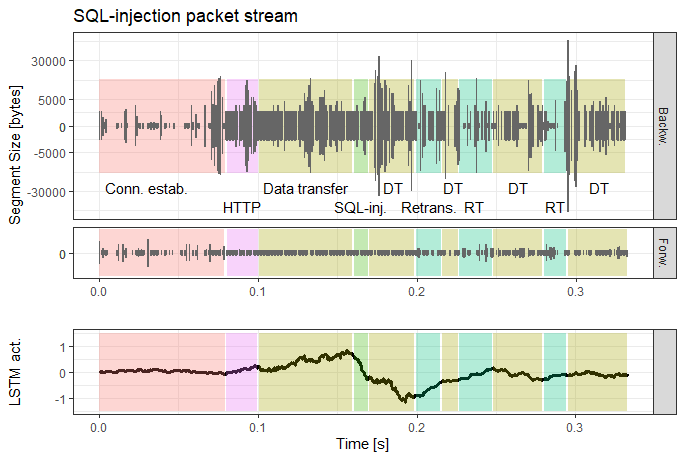
\includegraphics[width=0.5\textwidth]{images/LSTM_activation.png}
\caption{LSTM-output activation in dependence of connection phases. Depicted are packet segment streams and their respective sizes in the forward and backward direction, with different phases in the connection coloured and labelled. Below is the LSTM-ouput activation while processing the packet streams.}\label{fig:LSTM_act}
\end{figure}

The initially trained model overall performs relatively well, with an AUC-score\footnote{a measure describing the overall class separation of the model} of \textbf{0.981}, or a detection and false positive rate\footnote{tuned for the geometric mean} of \textbf{0.96\%} and \textbf{2.7\%}. However, we would ideally like to improve these rates to both detect more SQL-injections and retain a lower false-positive rate. We therefore begin to explore which type of connections are misclassified most. \textcolor{red}{potentially expand here to include influence of other traffic characteristics...}. For this, we rely on the various ground-truth information provided by DetGen for both the included malicious traffic as well as part of the benign traffic, that allow us to relate classification scores to simulated traffic characteristics. Looking at the left panel of Figure \ref{fig:LSTM_exp}, which depicts classification scores in dependence of the simulated network congestion, we learn that while classification scores are well separated for lower congestion, increased latency in a connection leads to a narrowing of the classification scores, especially for SQL-injection traffic. Since there are no classification scores that reach far in the opposing area, we conclude that congestion simply makes the model lose predictive certainty. A plausible cause would be that the increased amount of retransmission sequences decreases the overall sequential coherence for the model, i.e. that the LSTM-model loses context too quickly when processing retransmission sequences. 

To examine the exact effect of retransmission sequences on the model output, we generate two connections with the exact same characteristics except that one connection is subject to moderate packet loss and reordering while the other is not. We then compare how the LSTM-output activation is affected by retransmission sequences. Fig. \ref{fig:LSTM_act} depicts the evolution the LSTM-output layer activation in dependence of difference connection phases. As visible, initially the model begins to view the connection as benign when processing regular traffic, until the SQL-injection is performed. The model then quickly adjusts and provides a malicious classification after processing the injection phase and the subsequent data transfer. The negative output activation is however quickly depleted once the model processes a retransmission phase, and is afterwards not able to relate the still ongoing data transfer to the injection phase. When comparing this to the connection without retransmissions, we do not encounter this depletion effect, instead the negative activation persists after the injection phase.

We try to correct the existing model with a simple fix by excluding retransmission sequences from the model input data, which leads to significantly better classification results during network latency, as visible in the right panel of Figure \ref{fig:LSTM_exp}. SQL-injection scores are now far-less affected by congestion while scores for benign traffic are also less affected, albeit to a smaller degree.
The overall AUC-score for the model improves to \textbf{0.997} while tuned detection rates and false positives improved to \textbf{99.1\%} and \textbf{0.045\%}.


\begin{figure}
\centering
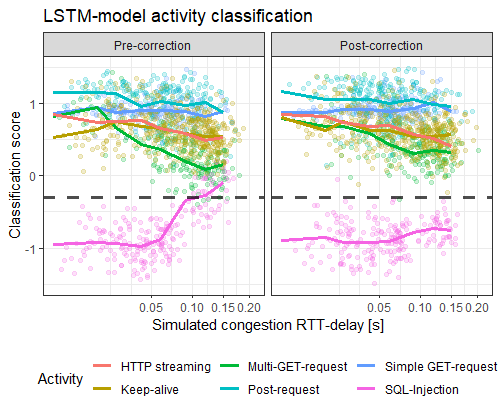
\includegraphics[width=0.5\textwidth]{images/LSTM_classi.png}
\caption{Scores for the LSTM-traffic classification model in dependence of simulated network congestion, along with the classification threshold. }\label{fig:LSTM_exp}
\end{figure}


%, so we should highlight their benefit most. Since ground-truth labels on attack data are existing in other datasets, we should emphasise the benefit of having labels for different activities. In my eyes, the most striking benefit arises for false-positive analysis, which we could then combine with showcasing the benefit of being able to generate different amounts of traffic for different activities.


%\paragraph{Plan}
%Implement the LSTM-model in the paper "An LSTM-Based Deep Learning Approach forClassifying Malicious Traffic at the Packet Level", train it on our data (both benign and attack traffic). Extract labels of traffic responsible for false-positives, show how much they are clustered around particular activities (potentially rare activities) compared to the overall traffic. Give potential reason for this. Generate a new dataset with increased amounts of the activities responsible for false positivies. Demonstrate that false-positives decrease.


\section{Refining the notion of benign traffic for anomaly detection}

Our second use-case looks at how ground-truth traffic information can help produce more coherent clusters and thus refine the capture of more detailed benign traffic structures in anomaly-detection. In particular, we will examine an anomaly-detection model by Casas et al. \cite{casas2012unsupervised} that produces state-of-the-art detection results for access attacks according to a survey by Nisioti et al. \cite{nisioti2018intrusion}.
The model takes a number of flow summary statistics as input, which include such as packet size and interarrival statistics, number of idle and transfer periods, flag occurrencies, number of flows in window, etc. as input and projects it into different subspaces, where the connections are clustered. Anomalous outliers are detected by accumulating the Mahalanobis-distance from the cluster centers from each subspace. The identified clusters therefore serve as structural enclosures of benign behaviour, with the cluster borders acting as separators to abnormal behaviours. Benign traffic should ideally be distributed evenly around the cluster centres to allow a tight borders and good separation from actual abnormal behaviour.

Unstructured datasets such as the CAIDA traffic traces assumably contain too much abnormal behaviour to train an anomaly-detection model, which is why we train the model on benign traffic from the CICIDS-17 intrusion detection dataset (80\%). Again, we also add traffic generated with the DetGen tool (HTTP, FTP, SSH, and SMTP, 20\%) using a wide spectrum of settings for examination purposes. Attack data for the evaluation was again provided through the CICIDS-17 dataset, and includes access attacks such as SQL-injections, Heartbleed, Brute-Force attacks etc. We  train the model with in total 15,000 connections.

\subsection{Projection coherency evaluation}

\begin{table}
\centering
\begin{tabular}{p{1cm}|p{2.3cm}|p{1.5cm}|p{1.6cm}}
Congest.&HTTP&File-Sync & Mirai-C\&C\\ \hline 
Low& Get-req. NGINX&  Two hosts & Command 1 \vspace{0.1cm} \\ \hline
1& \textcolor{myblue}{0.14}\space ,\space\space\textcolor{myred}{0.45} 
&\textcolor{myblue}{0.19}\space ,\space\space\textcolor{myred}{0.27} 
&\textcolor{myblue}{0.03}\space ,\space\space\textcolor{myred}{0.06}\\ \hline \hline
Low&Multi-req. NGINX & Four hosts & Command 2\\ \hline
2&\textcolor{myblue}{0.32}\space ,\space\space\textcolor{myred}{0.45} 
&\textcolor{myblue}{0.15}\space ,\space\space\textcolor{myred}{0.33} 
&\textcolor{myblue}{0.03}\space ,\space\space\textcolor{myred}{0.04}\\ \hline \hline
High& Post-req. Apache &Two hosts & Command 3\\ \hline
3&\textcolor{myblue}{0.17}\space ,\space\space\textcolor{myred}{0.28} 
&\textcolor{myblue}{0.16}\space ,\space\space\textcolor{myred}{0.28} 
&\textcolor{myblue}{0.02}\space ,\space\space\textcolor{myred}{0.04}\\ \hline \hline
High& Multi-req. Apache & Four hosts & Command 4\\ \hline
4&\textcolor{myblue}{0.53}\space ,\space\space\textcolor{myred}{2.51} 
&\textcolor{myblue}{0.71}\space ,\space\space\textcolor{myred}{1.31} 
&\textcolor{myblue}{0.03}\space ,\space\space\textcolor{myred}{0.05}\\ \hline \hline
\end{tabular}
\caption{Outline of the traffic settings evaluation, along with the average (blue) and maximal (red) Mahalanobis-distance for each projection.}\label{Tab:Dataset}
\end{table}

Like many approaches that generate representations of benign traffic for anomaly detection, Cases et al. project traffic events into a vector-space where traffic clusters and similarities become more apparent. In order for the projection to accurately capture important traffic structures, this projection should be consistent, i.e. traffic events with similar origins and characteristics should be projected to similar positions rather than be dispersed throughout the vector space. 

Verifying the projection consistency of a model is not straightforward as usually no or not enough ground-truth information about different traffic characteristics is available to asses if the model is projecting similar traffic to dissimilar positions, or if the traffic just bears some dissimilar characteristics.

Using DetGen, we are able to generate traffic from identical conditions to provide certainty on the expected traffic similarities, which is more suitable for the described task. We generate a small dataset that consists of traffic from 12 different settings, with the conducted activities and other traffic-shaping factors being held constant. Within each setting, we only allow for minor randomised effects such as packet reordering or slight variations in the activity input. Table \ref{Tab:Dataset} summarises the traffic from each setting. 


We verify if traffic samples within each group are projected to similar areas by measuring the average and maximum Mahalanobis-distance to quantify the overall dispersion of the samples. The results are displayed in Table \ref{Tab:Dataset} and depicted in Fig. \ref{fig:Subspace_disp}. First of all, the model projects all samples from each group within the same cluster, which confirms the capture of the coarse traffic structure. When looking at the traffic dispersion and the corresponding Mahalanobis-distance measurements, we notice that the \textit{multi-request HTTP} traffic as well as the \textit{file-synchronisation} between mutliple computers is much further dispersed than in the other settings, and that the corresponding axis with the most projected dispersion seems to be the same for each of the four settings, which suggests that the cause for the dispersion is the same for the different traffic types. When we look at the the influence of the individual flow features on projected position, we notice that even slight differences in the IAT of the preceding and the subsequent flow impacts the projected position quite strongly, which is why only the settings that generate multiple flows are affected.


\begin{figure}
\centering
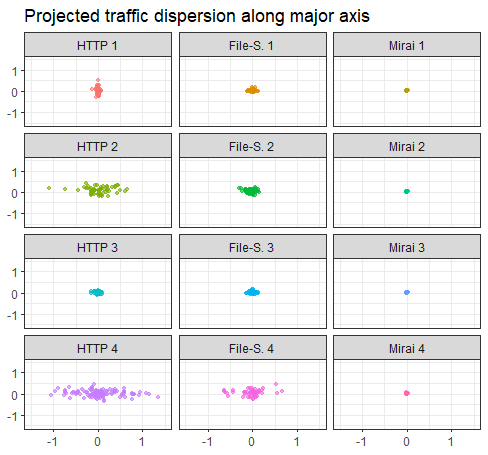
\includegraphics[width=0.5\textwidth]{images/traffic_dispersion.png}
\caption{Dispersion of projected traffic samples from each setting, plotted along the two most dispersed axes.}\label{fig:Subspace_disp}
\end{figure}


%at the effect of sudden connection terminations on an anomaly-detection model by Casas et al. \cite{casas2012unsupervised}. 

\subsection{Investigating individual cluster incoherences}

\begin{figure}
\centering
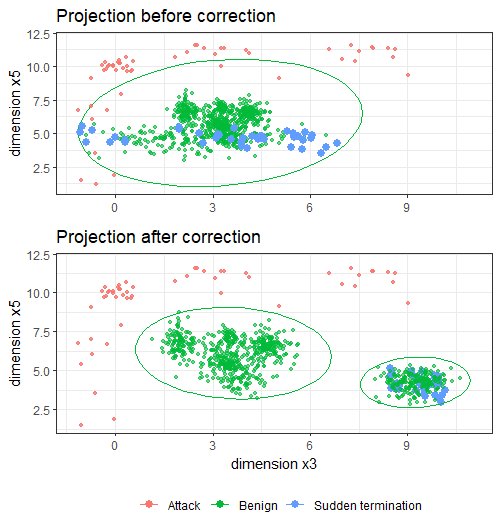
\includegraphics[width=0.5\textwidth]{images/Subspace_projection_new2.png}
\caption{Scores for the LSTM-traffic classification model in dependence of simulated network congestion, along with the classification threshold}\label{fig:Subspace_projection}
\end{figure}

When examining false-positive and corresponding anomaly scores, we noticed that in the CICIDS-17 dataset the model often classifies Brute-Force Web attacks as benign and some HTTP-traffic as anomalous. When examining the projected location of the corresponding connections, we see that most of this HTTP-traffic as well as the Brute-Force attack traffic lie near a particular cluster, depicted in Fig. \ref{fig:Subspace_projection}. A significant portion of traffic in that cluster seems to be spread significnatly more across the cluster axis than the rest of the traffic in that cluster, leading to an inflated radius that partially encompasses Brute-Force traffic. 

When cross-examining the traffic in this cluster with the DetGen traffic, we see that HTTP-traffic with the label "Sudden termination" are distributed across the cluster axis in a similar fashion, also depicted in Fig. \ref{fig:Subspace_projection}, suggesting the conclusion that this type of traffic causes the inflated cluster radius. DetGen generates traffic with the label "Sudden termination" as half-open connections which were dropped by the server due to network failure. One defining characteristic of such connections are that they are not closed with a termination handshake using FIN-flags. To better capture this defining characteristics in the modelling process, we included an additional feature that indicates a proper termination with FIN-flags in the modelling process. 

The newly trained model now projects "Sudden termination" connections into a different cluster, which leads to a far better cluster .

%In the evaluation of the model, it became apparent that the model often assigns Brute-Force Web attacks and some HTTP-traffic from a particular cluster similar anomaly scores. When looking at this cluster, we notice that despite most connections being well centred well together, some 
%connections are scattered much more broadly across the cluster and mix with Brute-Force traffic.
%This is visible in Figure \ref{fig:Subspace_projection}. When looking at the activity labels from DetGen, we notice that most of this traffic corresponds to half-open connections which were dropped by the server due to network failure. One defining characteristic of such connections are that they are not closed with a termination handshake using FIN-flags. We therefore included an additional flow-summary describing whether the connection was terminated properly, which lead to half-open connections being projected very differently into a new cluster with well defined borders.


%\subsection{Verifying model performance against adversarial perturbations}
%Investigating adversarial perturbation attacks and model inversion}

%Recently, research to verify intrusion detection model output has gained interest in order to provide guarantees for the detection of specific attacks or against flagging certain benign events as malicious, and especially verifying robustness against traffic perturbations is seen as a pressing issue. 
%We look at a simple neural network classifier designed to detect HTTP Brute-Force attacks. Our aim is to verify the robustness of the model performance against artificial packet interarrival perturbations that an attacker could introduce to  alter the classification result. 
%To test the trained model, we generated traffic from a Brute-Force attack scenario to which we added jitter delays with varying amounts and drawn from varying distributions. 
%\cite{kokke2020neural}
%\textcolor{red}{insert results}


%
%\subsection{\textcolor{red}{Empirical} evaluation of traffic sequence embeddings}
%
%Recently, the embedding of sequences into a vectorised representation has gained traction in the \textcolor{red}{network science community} \cite{gonzalez2017net2vec,lin2019generating}. Embeddings are \textcolor{red}{(often low-dimensional)} vectors that aim to characterise a sequence through its position in a vector space. This numerical representation can then be used in various ways, such  as to classify or cluster traffic, profile hosts or users, or generate new artificial traffic traces. 
%
%Since the embedded position of a traffic relative to similar or dissimilar traffic  crucial \textcolor{red}{...}
%
%In this use-case, we are examining the Net2Vec-model by Gonzalez et al. \cite{gonzalez2017net2vec} and the corresponding embeddings it generates.
%
%\subsubsection{Position consistency evaluation}
%
%It is absolutely crucial for a represenation model that sequences with the same characteristics receive a similar embedding, i.e. traffic traces that correspond to the same activity and settings should be projected very close together. 
%
%To do so, we generate traffic from settings within which all controllable influence factors are held constant. Traffic samples from each setting should then be similar up to small deviations in IATs, additional ACK-packets etc., such as depicted in Fig. \ref{Fig:HTTP_ex}. \textcolor{red}{The different traffic sample groups are listed in Table \ref{Tab:Dataset}.
%
%\begin{figure}
%\centering
%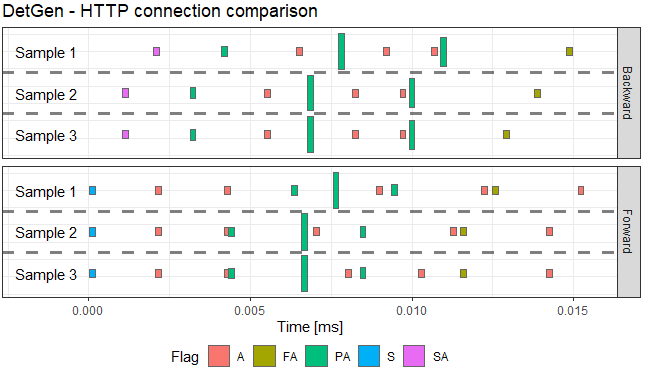
\includegraphics[width=0.45\textwidth]{images/HTTP_ex.png}
%\caption{Packet-sequence structure similarity comparison for HTTP-activity under constant settings generated by the DetGen framework (left) and in a regular setting (right). Colours indicate packet flags while the height of the packets indicates their size. Note that in addition to more differences in the timing, the packet sizes vary more in the regular setting. }\label{Fig:HTTP_ex}
%\end{figure}
%
%We now examine the positions that 
%
%\begin{table}
%\centering
%\begin{tabular}{p{1cm}|p{1cm}|p{2.7cm}|p{1.5cm}|p{2.7cm}}
%Label &Congest.&HTTP&File-Sync & Mirai-C\&C\\ \hline
%A&Low& Get-req. NGINX&  Two hosts & Command 1 \\ \hline
%DetGen &&\footnotesize \textcolor{myred}{0.20\%}, \textcolor{mygreen}{0.03\%}, \textcolor{myblue}{0.18\%}&
% \footnotesize \textcolor{myred}{0.12\%}, \textcolor{mygreen}{0.01\%}, \textcolor{myblue}{0.19\%}&
% \footnotesize \textcolor{myred}{0.21\%}, \textcolor{mygreen}{0.0\%}, \textcolor{myblue}{0.22\%}\\ \hline \hline
%%VM & &\footnotesize \textcolor{myred}{1.5\%}, \textcolor{mygreen}{3.8\%}, \textcolor{myblue}{1.3\%}& \footnotesize \textcolor{myred}{0.9\%}, \textcolor{mygreen}{1.6\%}, \textcolor{myblue}{0.38\%}& \footnotesize \textcolor{myred}{1.1\%}, \textcolor{mygreen}{1.8\%}, \textcolor{myblue}{0.7\%}\\ \hline \hline
%B& Low&Multi-req. NGINX & Four hosts & Command 2\\ \hline
%DetGen &&\footnotesize \textcolor{myred}{0.27\%}, \textcolor{mygreen}{0.30\%}, \textcolor{myblue}{0.17\%}&
%\footnotesize \textcolor{myred}{0.11\%}, \textcolor{mygreen}{0.1\%}, \textcolor{myblue}{0.24\%}&
%\footnotesize \textcolor{myred}{0.19\%}, \textcolor{mygreen}{0.02\%}, \textcolor{myblue}{0.17\%}\\ \hline \hline
%%VM & &\footnotesize \textcolor{myred}{1.3\%}, \textcolor{mygreen}{2.9\%}, \textcolor{myblue}{0.9\%}& \footnotesize \textcolor{myred}{1.1\%}, \textcolor{mygreen}{4.9\%}, \textcolor{myblue}{1.2\%}& \footnotesize \textcolor{myred}{1.1\%}, \textcolor{mygreen}{1.1\%}, \textcolor{myblue}{0.6\%}\\ \hline \hline
%C& High& Post-req. Apache &Two hosts & Command 3\\ \hline
%DetGen &&\footnotesize \textcolor{myred}{0.41\%}, \textcolor{mygreen}{0.01\%}, \textcolor{myblue}{0.29\%}&
% \footnotesize \textcolor{myred}{0.39\%}, \textcolor{mygreen}{0.01\%}, \textcolor{myblue}{0.21\%}&
% \footnotesize \textcolor{myred}{0.29\%}, \textcolor{mygreen}{0.02\%}, \textcolor{myblue}{0.23\%}\\ \hline \hline
%%VM & &\footnotesize \textcolor{myred}{1.9\%}, \textcolor{mygreen}{1.3\%}, \textcolor{myblue}{1.5\%}& \footnotesize \textcolor{myred}{1.3\%}, \textcolor{mygreen}{1.4\%}, \textcolor{myblue}{1.2\%}& \footnotesize \textcolor{myred}{1.1\%}, \textcolor{mygreen}{1.3\%}, \textcolor{myblue}{0.9\%}\\ \hline \hline
%D& High& Multi-req. Apache & Four hosts & Command 4\\ \hline
%DetGen &&\footnotesize \textcolor{myred}{0.55\%}, \textcolor{mygreen}{0.39\%}, \textcolor{myblue}{0.20\%}&
% \footnotesize \textcolor{myred}{0.31\%}, \textcolor{mygreen}{0.15\%}, \textcolor{myblue}{0.38\%}&
% \footnotesize \textcolor{myred}{0.24\%}, \textcolor{mygreen}{0.0\%}, \textcolor{myblue}{0.32\%}\\ \hline \hline
%%VM & &\footnotesize \textcolor{myred}{1.9\%}, \textcolor{mygreen}{4.2\%}, \textcolor{myblue}{1.4\%}& \footnotesize \textcolor{myred}{1.6\%}, \textcolor{mygreen}{4.8\%}, \textcolor{myblue}{1.4\%}& \footnotesize \textcolor{myred}{0.9\%}, \textcolor{mygreen}{1.2\%}, \textcolor{myblue}{0.9\%}\\ \hline \hline
%\end{tabular}
%\caption{Outline of the traffic settings used for the determinism evaluation, along with the average dissimilarity percentages for each setting (red=overall connection similarity, green=connection sequence similarity, blue=packet sequence similarity)}\label{Tab:Dataset}
%\end{table}
%
%
%
%\subsubsection{Similarity evaluation}
%
%
%
%
%\section{Fidelity confirmation experiments}\label{Sec:Experiments}
%
%%This section is important to demonstrate that our data is valid and overcomes the difficulties entailed with synthetic data generation. Cordero et al. have proposed some more simple test that we can refer to first
%
%%\textcolor{red}{Question to be answered}: What requirements are there for the additional data, program logs and system logs, that we collect? Should we put less emphasise on these data sources in general if we are not able to perform these tests, and refer to them in future work? I am not aware of any papers that discuss these requirements in a similar way. 
%
%
%%\subsection{Traffic similarity metrics for determinism and realism evaluation}
%\subsection{Traffic control and generation determinism}
%We now assess the claim of control over the outlined traffic influence factors, and how similar traffic generated with the same settings looks like. We also demonstrate that this level of control is not achievable on regular VM-based NIDS-traffic-generation setup.
%
%To do so, we generate traffic from settings within which all controllable influence factors are held constant, both with DetGen framework and with a regular VM-based setup. Traffic samples from each setting should then be as similar as possible to provide sufficient experimental determinism. To measure how similar two traffic samples are, we devise a set of similarity metrics that measure dissimilarity of overall connection characteristics, connection sequence characteristics, and packet sequence characteristics:
%
%
%\begin{figure}
%\centering
%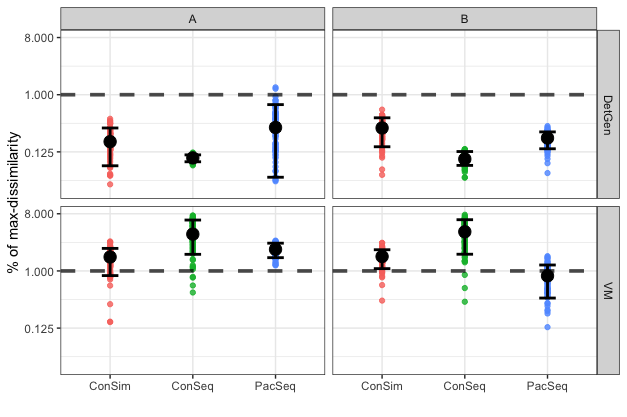
\includegraphics[width=0.5\textwidth]{images/Exp1.png}
%\caption{Comparison of HTTP-group dissimilarity scores for the DetGen-framework and a regular VM-setup, on a logarithmic scale. Samples from the VM-setting are consistently more dissimilar, in particular for flow-based metrics, where the average dissimilarity is more than 30 times higher than for the DetGen setting.}\label{Fig:determ-metric}
%\end{figure}
%
%
%%To do so, we require a similarity metric that measures how similar or dissimilar two traffic traces are. We want to compare traffic similarity on three ...
%%we compare our framework against a setup on a virtual machine to show that we provide deterministic control that is not achievable on a common setup. 
%%For that, we measure traffic similarity using a set of similarity metrics on traffic both from our and the comparison setup. The traffic is subject to varying degrees of influence from the above described impact factors. We show that when all factors are held constant, our traffic is much more similar than on a regular setup.
%
%%We should also demonstrate how difficult it is to match all flow events to specific events (I am still unsure how), and how often you get system background events (very straightforward using flow counting and port entropy).
%
%%Common setup: Network of VMs with each VM representing one host in a regular network. Multiple services with scheduled scripted activities running on a VM. Traffic captured at router or network interface. 
%
%\begin{itemize}
%\item \textbf{Overall connection similarity} We collect 80 flow summary statistics (IAT and packet size, TCP window sizes, flag occurrences, burst and idle periods). We compress this information using PCA to 8 significant dimensions, and measure the cosine similarity between connections, which is also used in general traffic classification \cite{aun2017review}.
%\item \textbf{Connection sequence similarity} 
%To quantify the similarity of a sequence of connections in a retrieval window, we use the following features to describe the window, such as used by Yen et al. \cite{yen2009browser} for application classification: The number of connections, average and max/min flow duration and size, number of distinct IP and ports addresses contacted. We then again measure the cosine similarity based on these features between different windows. 
%\item \textbf{Packet sequence similarity} To quantify the similarity of packet sequences in traffic captures, we assign packets a discrete state according to their flags, direction, sizes, and interarrival times (\textcolor{red}{insert citation}). We then calculate the Markovian probability of each packet state conditional on the previous packet. We do this for sequences of 15 packets at the start, the middle, and the end of a connection, and use the average sequence likelihood of each group as a similarity measure. If connections are completely similar, the conditional probabilities and thus the likelihoods should converge to one.
%\end{itemize}
%
%We normalise all dissimilarity scores by dividing them by the maximum dissimilarity score measured for each traffic type in our experiment in Section \ref{Sec:Realdiv}, so that the reader can relate the measured scores to the traffic type.
%
%
%
%\begin{table*}
%\centering
%\begin{tabular}{p{1cm}|p{3.2cm}|p{2.7cm}|p{2.7cm}|p{2.7cm}}
%Label &Overall Setting&HTTP&File-Sync & Mirai-C\&C\\ \hline
%A&Low congest., high load& Get-req. NGINX&  Two computers & Command seq. 1 \\ \hline
%DetGen &&\footnotesize \textcolor{myred}{0.20\%}, \textcolor{mygreen}{0.03\%}, \textcolor{myblue}{0.18\%}&
% \footnotesize \textcolor{myred}{0.12\%}, \textcolor{mygreen}{0.01\%}, \textcolor{myblue}{0.19\%}&
% \footnotesize \textcolor{myred}{0.21\%}, \textcolor{mygreen}{0.0\%}, \textcolor{myblue}{0.22\%}\\ \hline \hline
%VM & &\footnotesize \textcolor{myred}{1.5\%}, \textcolor{mygreen}{3.8\%}, \textcolor{myblue}{1.3\%}&
% \footnotesize \textcolor{myred}{0.9\%}, \textcolor{mygreen}{1.6\%}, \textcolor{myblue}{0.38\%}&
% \footnotesize \textcolor{myred}{1.1\%}, \textcolor{mygreen}{1.8\%}, \textcolor{myblue}{0.7\%}\\ \hline \hline
%B& Low congest., no load &Multi-req. NGINX & Four computers & Command seq. 2\\ \hline
%DetGen &&\footnotesize \textcolor{myred}{0.27\%}, \textcolor{mygreen}{0.30\%}, \textcolor{myblue}{0.17\%}&
%\footnotesize \textcolor{myred}{0.11\%}, \textcolor{mygreen}{0.1\%}, \textcolor{myblue}{0.24\%}&
%\footnotesize \textcolor{myred}{0.19\%}, \textcolor{mygreen}{0.02\%}, \textcolor{myblue}{0.17\%}\\ \hline \hline
%VM & &\footnotesize \textcolor{myred}{1.3\%}, \textcolor{mygreen}{2.9\%}, \textcolor{myblue}{0.9\%}&
% \footnotesize \textcolor{myred}{1.1\%}, \textcolor{mygreen}{4.9\%}, \textcolor{myblue}{1.2\%}&
% \footnotesize \textcolor{myred}{1.1\%}, \textcolor{mygreen}{1.1\%}, \textcolor{myblue}{0.6\%}\\ \hline \hline
%C& High congest., no load & Post-req. Apache &Two computers & Command seq. 3\\ \hline
%DetGen &&\footnotesize \textcolor{myred}{0.41\%}, \textcolor{mygreen}{0.01\%}, \textcolor{myblue}{0.29\%}&
% \footnotesize \textcolor{myred}{0.39\%}, \textcolor{mygreen}{0.01\%}, \textcolor{myblue}{0.21\%}&
% \footnotesize \textcolor{myred}{0.29\%}, \textcolor{mygreen}{0.02\%}, \textcolor{myblue}{0.23\%}\\ \hline \hline
%VM & &\footnotesize \textcolor{myred}{1.9\%}, \textcolor{mygreen}{1.3\%}, \textcolor{myblue}{1.5\%}&
% \footnotesize \textcolor{myred}{1.3\%}, \textcolor{mygreen}{1.4\%}, \textcolor{myblue}{1.2\%}&
% \footnotesize \textcolor{myred}{1.1\%}, \textcolor{mygreen}{1.3\%}, \textcolor{myblue}{0.9\%}\\ \hline \hline
%D& High conges., high load & Multi-req. Apache & Four computers & Command seq. 4\\ \hline
%DetGen &&\footnotesize \textcolor{myred}{0.55\%}, \textcolor{mygreen}{0.39\%}, \textcolor{myblue}{0.20\%}&
% \footnotesize \textcolor{myred}{0.31\%}, \textcolor{mygreen}{0.15\%}, \textcolor{myblue}{0.38\%}&
% \footnotesize \textcolor{myred}{0.24\%}, \textcolor{mygreen}{0.0\%}, \textcolor{myblue}{0.32\%}\\ \hline \hline
%VM & &\footnotesize \textcolor{myred}{1.9\%}, \textcolor{mygreen}{4.2\%}, \textcolor{myblue}{1.4\%}&
% \footnotesize \textcolor{myred}{1.6\%}, \textcolor{mygreen}{4.8\%}, \textcolor{myblue}{1.4\%}&
% \footnotesize \textcolor{myred}{0.9\%}, \textcolor{mygreen}{1.2\%}, \textcolor{myblue}{0.9\%}\\ \hline \hline
%\end{tabular}
%\caption{Outline of the traffic settings used for the determinism evaluation, along with the average dissimilarity percentages for each setting (red=overall connection similarity, green=connection sequence similarity, blue=packet sequence similarity)}\label{Tab:Dataset}
%\end{table*}
%
%
%%\subsubsection{Determinism test}
%As a comparison, we use a regular VM-based setup, were applications are hosted directly on two VMs that communicate over a virtual network bridge that is subject to the same NetEm effects as DetGen. To compare the amount of traffic control and the corresponding generative determinism of DetGen and the VM-setup, we generate three different types of traffic (HTTP, file-syncing, and botnet) from four different settings, within which all generative parameters are kept constant. For each setting and traffic type, we generate 100 traffic samples and apply the described dissimilarity measures to 100 randomly drawn pairs sample pairs. Fig. \ref{Fig:determ-metric} depicts the calculated dissimilarity scores for DetGen and the VM-setup, while Table \ref{Tab:Dataset} describes the different settings and the corresponding average dissimilarity scores.
%
%As visible, the scores yield less than $1\%$ of the dissimilarity observed on average for each protocol. Scores are especially low when compared to traffic groups collected in the VM setting, which is also visible in Fig. \ref{determ-metric} for the HTTP-traffic. Dissimilarity scores for the VM-setting are most notably higher for the flow-metric, caused by additional background flows frequently captured. While sequential dissimilarity is roughly the same for the DetGen- and the VM-settings, overall connection similarity for the VM-setting sees significantly more spread in the dissimilarity scores when computational load is introduced.
%
%
%%We now apply the described similarity measures to different settings of traffic traces to evaluate the \textcolor{red}{determinism} of our data generation process. We vary the control settings of the described influence factors, described in Section \ref{Sec:Impactfactors}, for each group, but keep them constant within each group. We use three different traffic types (HTTP, file-syncing (port 8384), and botnet), for which we both perform different application-specific activities and create different overall settings. 
%
%%We furthermore perform the same HTTP-activities on two regular VMs without containerisation, but with the same settings.
%
%
%\begin{figure}
%\centering
%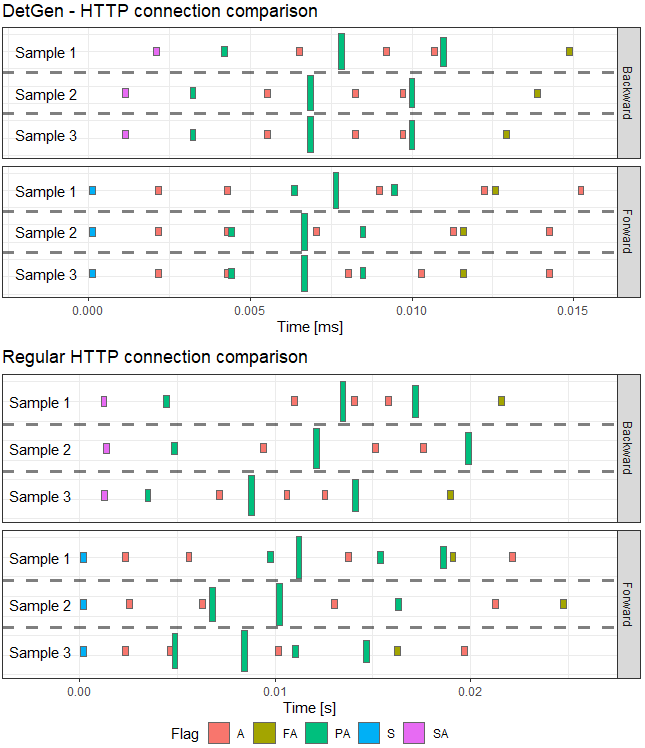
\includegraphics[width=0.45\textwidth]{images/HTTP_comp_crop.png}
%\caption{Packet-sequence structure similarity comparison for HTTP-activity under constant settings generated by the DetGen framework (left) and in a regular setting (right). Colours indicate packet flags while the height of the packets indicates their size. Note that in addition to more differences in the timing, the packet sizes vary more in the regular setting. }
%\end{figure}

%Table \ref{Dataset} summarises the activity and settings for the different traffic groups, along with the corresponding dissimilarity scores for each group. 


%0.2043341 0.2099933 0.1892661 0.2779625 0.3052004 0.1835523 0.4104484 0.3933690 0.2935111 0.5524176 0.1028654 0.2028906 2.6549903 3.4444166 2.2215654





%\subsection{Realistic diversity level evaluation}\label{Sec:Realdiv}

%The above test demonstrated that while holding settings constant, DetGen generates traffic with high similarity. We now prove that this does not impede DetGen's capability to generate realistic amounts of traffic diversity observed in real-world traffic. This is an important issue since low diversity in training data can both lead to overfitting and to less generalizable models, which can inflate test results compared to real-world settings. However, a lack of traffic diversity and overly homogeneous traffic is inherent to all current intrusion detection datasets \cite{sommer2010outside}.

%An illustrative example of this restricted protocol activity in synthetic datasets can be seen in the CICIDS 2017 dataset \textcolor{red}{insert citation}. Here, the vast majority of successful HTTP transfers consist of a client downloading a single text file containing the Wikipedia page for `Encryption' several hundred times in a day. In reality, HTTP is used for a large number of tasks, which can occur in random order with varying input sizes and parameters.


%For our examination, we create a mixed dataset with varying settings for each protocol to explore the produced traffic diversity. Again, we use the proposed traffic similarity metrics to measure the overall traffic dissimilarity. 
%We compare the observed dissimilarity for each protocol with that observed in real-world traffic from the CAIDA-2018 anonymized traffic traces \textcolor{red}{insert citation}, as well as the widely used synthetic CICIDS-17 intrusion detection dataset \textcolor{red}{insert citation}. Ideally, our generated traffic exhibits similar overall traffic diversity as the CAIDA real-world traffic.



%\begin{figure}
%\centering
%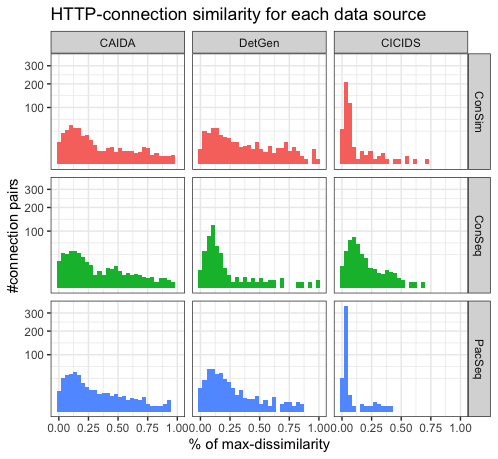
\includegraphics[width=0.5\textwidth]{images/HTTP_similarity.png}
%\caption{HTTP-traffic dissimilarity scores for each metric and each of the datasets.}\label{fig:diversity_exp}
%\end{figure}
%
%We examine the achievable traffic diversity for HTTP-traffic, since large amounts of this protocol are present both in the CAIDA and the CICIDS-17 dataset.
%We randomly draw settings for all impact factors simultaneously during the traffic generation using realistic parameter sampling distributions, as described in Section \ref{Sec:Scenarios}. After the traffic collection, we pair HTTP-connections at random to examine their dissimilarity. 
%
%Figure \ref{fig:diversity_exp} shows the dissimilarity distribution for the three traffic metrics for each dataset. As visible, neither the data from DetGen nor the CICIDS-17 dataset fully achieves the diversity of the CAIDA-data. However, DetGen achieves significantly more diversity for overall connection features and for packet sequences, areas whereas the data in the CICIDS-17 data is clustered very narrowly. Normalised entropy measures to quantify the spread of the score distributions for the CAIDA dataset are (\textcolor{myred}{8.14}, \textcolor{mygreen}{8.24}, and  \textcolor{myblue}{8.16}), whereas the DetGen framework achieves entropy scores of (\textcolor{myred}{8.02}, \textcolor{mygreen}{6.6}, and  \textcolor{myblue}{7.91}) while the CICIDS-17 dataset only achieves (\textcolor{myred}{4.3}, \textcolor{mygreen}{6.7}, and  \textcolor{myblue}{2.5})\footnote{Colours correspond to the respective similarity measure.}. This shows that by varying traffic control parameters in a controlled manner, DetGen edges significantly closer to real-world traffic for both overall connection similarity and packet sequence similarity, and performs similarly to existing methods for connection sequence similarity. 

% and test if the traffic similarity scores are as divergent as for traffic from a real-world dataset (i.e. CAIDA) for two or three exemplary protocols, and we also compare it to the same protocols in the CICIDS-17 dataset. This will let us argue that we can achieve realistic levels of diversity (something criticised by Sommer-Paxson), and that our framework lets researchers explore higher levels of diversity than currents labelled solutions.



%\subsection{Data correctness tests}

%This section is concerned with dataset defects, artifacts, or invalid data (inconsistent MTU etc.). These are very straightforward to test and should not take up much space. 


%\subsection{Diversity tests}

%These tests, also from Cordero et al. quantify diversity via the entropy of different quantities such as IP diversity, Time-to-Live, Maximum-segment-size, Window size, ToS. I think we should keep this relatively short and omit comparison to other datasets since this is already done by Cordero et al. 


%\subsection{Structural dataset dimensionality}



%Autoencoders are often used to compress non-deterministic, noisy data. Bahadur et al. have developed a procedure to estimate the ,,dimensionality'' (to be understood as the complexity) of a dataset using variational autoencoders. I believe we can transfer this concept to sequence compression and estimate the overall complexity of connection sequences in our framework with both real traffic captures and existing network intrusion datasets. 

%Showing that our data is closer to real-world data would be a good test for "artificially predictable patterns", as described by Cordero et al., and go hand-in-hand with demonstrating the benefits of our framework for the training of deep-learning models. The importance of data that is less artificially predictable and closer to real-life traffic in terms of statistical variations lies in its suitability as a benchmark for detection rates, since less complex data is easier to train on and yields unrealistically high detection rates. 


%Measure structural richness of
%Also measure divergence across same activities (same activity and same port)
%Demonstrate benefit of structural richness
%Closer to reality



%\subsection{Reproducible scenarios}\label{Sec:deterministic}

%\dots \dots

%\dots \dots

%\dots \dots
%\begin{figure}
%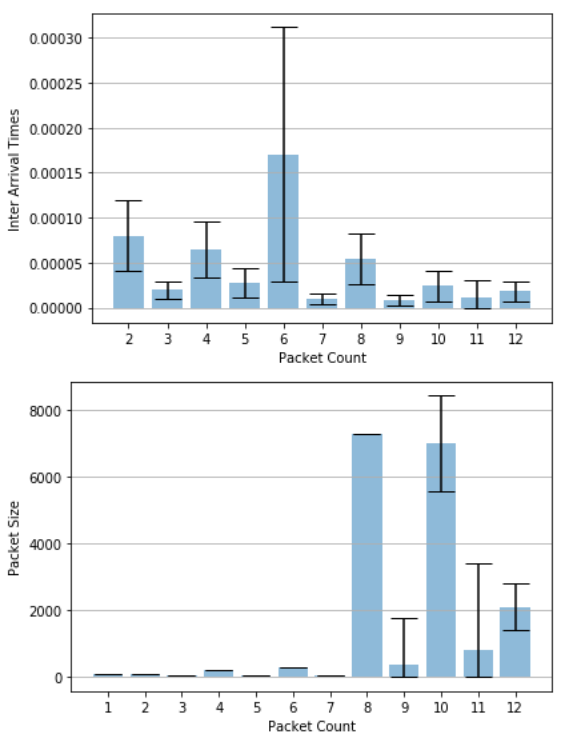
\includegraphics[width=0.45\textwidth]{images/combined3.png} % first figure itself
%\caption{Means of IATs \& packet sizes along with standard deviation bars for the first twelve packets in the Apache scenario.}
%\label{fig:size1}
%\end{figure}

 


% Need to edit these sections to provide a single context for both the artificial delays & classification

%\subsection{Explorating Artificial Delays}

%This section is already existing, we could potentially expand this. I think it is sufficient and analysing it more does not add much to the paper as the performance of TC netem is relatively well accepted. I think we could even move this section to the appendix.

%\begin{figure}
%\captionsetup{justification=centering}
%\centering
%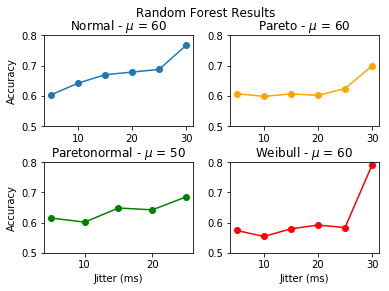
\includegraphics[width=0.45\textwidth]{images/1-plot_exp1.png}
%\caption{Results of Random Forest Classifier for a given distribution at the best performing delay mean $\mu$. Note that a score of .5 indicates total indistinguishability.}
%\label{Fig:rf_graph}
%\end{figure}
%
%
%
%\begin{table}[ht!]
%\begin{center}
%\begin{small}
%\begin{sc}
%\begin{tabular}{ccccc}
%\hline
%Distribution & Mean & Jitter & RF Accuracy\\
%\hline
%No Delays (Baseline) & 0 & 0ms & 0.8176 \\
%Constant Delay & 40ms & 0ms & 0.6730 \\
%Normal & 60ms & 5ms & 0.6028 \\
%Pareto & 60ms & 10ms & 0.5979 \\
%Paretonormal & 50ms & 10ms & 0.6015 \\
%Weibull & 60ms & 10ms & 0.5540 \\
%\hline
%\end{tabular}
%\end{sc}
%\end{small}
%\caption{Worst Random Forest accuracy rates for a given distribution}
%\label{tab:results-iat_rf}
%\end{center}
%\vskip -4mm
%\end{table}



%\subsubsection{Benefits of structural richness}
%
%Possible title: \textbf{Harder benchmarks}
%
%As described above, the importance of data that is less artificially predictable and closer to real-life traffic in terms of statistical variations lies in its suitability as a benchmark for detection rates. In particular, we want to demonstrate that our data functions is a more difficult and realistic benchmark that is less prone to inflating detection rates than existing datasets, something that is often a point of criticism for models evaluated on synthetic data. 
%
%To show that the training and detection is harder on our data, we could generate a dataset with similar attacks and services as the CICIDS-17 dataset, and train the above described LSTM model on both datasets. We could show that the training loss goes down more slowly on our data, as well as other metrics (increased validation loss --> overfitting etc.). We could then go ahead and show that the same attacks are detected easier by the same model in the CICIDS-17 data than in our data, concluding that it is a less realistic benchmark.
%
%It would be good to also include a comparison with actual real-world traffic here to bolster our conclusion, but due to the lack of structured real-life datasets it is difficult to create a fair and scientific comparison. 
%
%%\subsubsection{Show utility of tuning amount of rare events}
%
%\subsection{Show utility of flexible topology}
%
%This is another possibility to demonstrate that the flexibility provided through containerisation allows for better benchmarking and more in-depth evaluation.
%
%Methods aiming at modelling network structures are an established method for botnet and pivoting detection. Even though the network topology is a crucial variable in their training, their evaluation is to my knowledge only done on single static datasets such as the LANL-15. 
%
%My idea is that we generate about 10 datasets with different topologies, (especially different numbers of subnets and servers), and highlight the variation in prediction accuracy, i.e. the accuracy on one dataset is significantly higher/lower, and the average across the different datasets is a better indicator that eliminates the topology as a variable. We do not necessarily need to implement any attack traffic here since the modelling accuracy on benign traffic should be sufficiently quantifiable. 
%
%A suitable candidate for the evaluation would be the paper "Link prediction in dynamic networks using randomdot product graphs", which comes from people at Imperial College that I know. The model tries to give a probability for each connection to appear in a network, in order to spot connections between unlikely pairs as anomalous behaviour. I could ask the people for the implemented model so we do not have to do it ourselves, or we could even have a chat with them.
%
%
%%\begin{figure}%[ht!]
%%\subfloat{%
%% 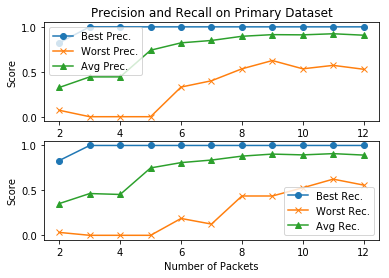
\includegraphics[width=0.4\textwidth]{images/bw_100_exp_3.png}}
%%\subfloat{
%% 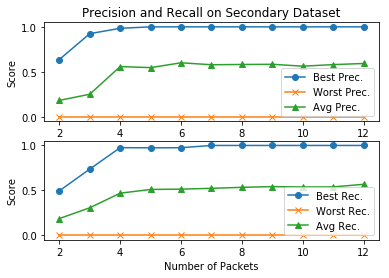
\includegraphics[width=0.4\textwidth]{images/bw_500_exp_3.png}}
%%\caption{Results of Random Forest Classification on Primary dataset (Above) and Secondary dataset (Below)}
%%\label{Fig:Primary}
%%\end{figure}
%
%\subsection{Customisable attack traffic by using metasploitable}
%
%Rob and I discussed that by using a combination of a metasploit-attack container and a metasploitable-victim container, we could generate and embed a significantly larger number of attack traffic types more efficiently than we are currently. Since we can attach the metasploitable-container to the network interface of regular containers, we can embed the implemented vulnerabilities very easily in a given scenario. Furthermore, since both containers are well maintained, we can keep the attack catalogue up-to-date.
%
%I think the best use-case is to showcase the process of adding a new type of attack to the dataset, embedding it in a proper way to a given scenario, generating data from it. We could additionally implement a corresponding detection method, but I think this would not demonstrate anything. 
%
%
%\subsection{Simple use-case for the microservice mode?}
%This use-case depends a lot on the state of the framework, but we could in principle show the benefits of the framework for the recently published model in "AppMine: Behavioral Analytics for Web Application Vulnerability Detection" on a more extensive dataset, since they only had very limited data available. 
%\section{Conclusions}\label{Sec:Conclusion}
%
%
%
%\subsection{Difficulties and limitations}



%\section{Impact factors on traffic micro-structures}\label{Sec:Impactfactors}
%
%In order to enable sufficient and reproducible control over the generated traffic and provide the corresponding descriptive ground truth information , we first must understand what factors shape the traffic generation process. 
%Computer communication involves a myriad of different computational aspects, and no research so far has been conducted to quantify how much influence each of them has on traffic structures. The following list highlights the most important influence factors on the traffic micro-structures observed on individual devices, as shown by other researchers or our own experiments:
%\textcolor{red}{How do we verify that this list is more or less complete?}
%
%\paragraph{1. Application layer protocols} 
%Without doubt the biggest impact on the captured traffic micro-structures is the choice or combination of the application layer protocols. Protocols such as HTTP/TLS perform vastly different tasks than protocols such as Peer-2-Peer or SMB, and thus perform different handshakes, experience different waiting times, transfer data in different intervals, or trigger different additional connections. 
%
%%\begin{figure}
%%\centering
%%\begin{subfigure}[b]{0.46\textwidth}
%%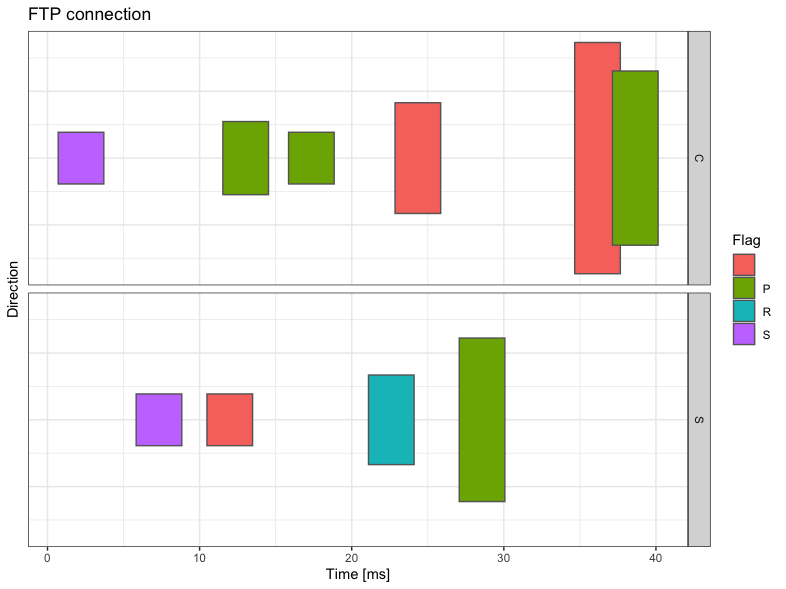
\includegraphics[width=\textwidth]{images/FTP.png}
%%\caption{Packet sequence in FTP connection}
%%\end{subfigure}
%%~
%%\begin{subfigure}[b]{0.46\textwidth}
%%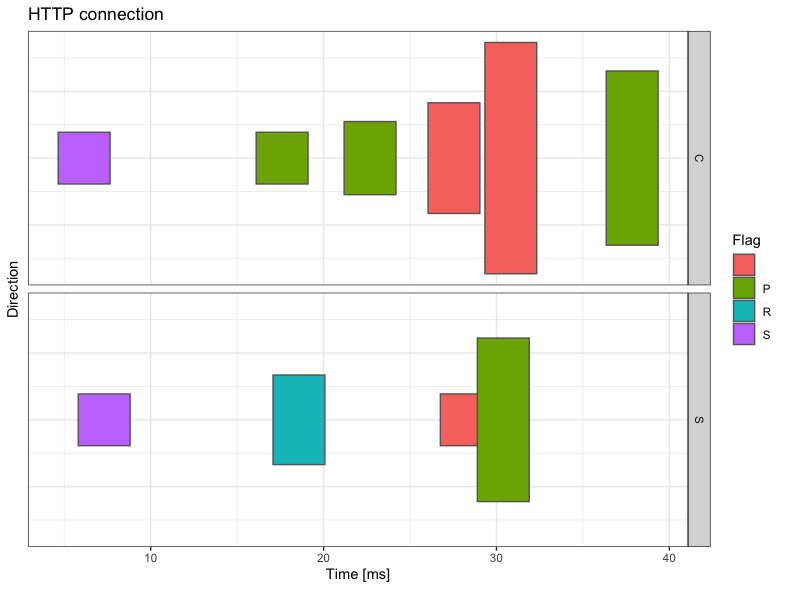
\includegraphics[width=\textwidth]{images/HTTP.png}
%%\caption{Packet sequence in HTTP connection}
%%\end{subfigure}
%%\end{figure}
% 
%\paragraph{2. Performed task and application}
%The conducted computational task ultimately drives the communication between computers, and thus hugely influences characteristics such as the direction of data transfer, the duration and packet rate, packet sizes as well as the number of connections and performed protocol handshakes to conclude the task. Furthermore, the application used for the task has a significant influence on the generated traffic, as shown for different browser choices by Yen et al. \cite{yen2009browser} or for general application behaviour fingerprinting \cite{stober2013you}. 
%
%\paragraph{3. Transferred data} 
%The amount of transferred data influences the overall packet numbers. Furthermore, the content of the data can potentially impact packet rates and sizes, such as shown by Biernacki \cite{biernacki2017analysis} for streaming services.
%
%
%\begin{table}[h!]
%\centering
%\begin{tabular}{l|l|l|>{\bfseries}l}
%Time&  Source-IP &Destination-IP& Dest. Port\\ \hline
%13:45:56.8 & 192.168.10.9 &  192.168.10.50 &       21 \\ \hline
%13:45:56.9 & 192.168.10.9 &  192.168.10.50 &    10602\\ \hline
%13:45:57.5 & 192.168.10.9 &  69.168.97.166 &      443\\ \hline
%13:45:59.1 & 192.168.10.9 &   192.168.10.3 &       53\\ \hline
%13:46:00.1 & 192.168.10.9 & 205.174.165.73 &     8080\\ \hline
%\end{tabular}
%\caption{Exemplary activity interval for host 192.168.10.9 in the CICIDS-17 dataset, containing FTP-, HTTPS- and DNS-, as well as additional unknown activity.}\label{Tab:Sess}
%\end{table}
%
%\paragraph{4. Caching/Repetition effects}
%Tools like cookies, website caching, DNS caching, known hosts in SSH, etc. remove one or more information retrieval requests from the communication, which can lead to altered packet sequences, less connections being established. For caching, this can result in less than $10\%$ of packets being transferred, as shown by Fricker et al. \cite{fricker2012impact}. 
%
%% parts of a communication being skipped and lead to differences in the captured traffic between initial and subsequent connections.
%
%
%
%\paragraph{5. Captured traffic from background activity} 
%In traditional setups, all traffic generated on a host is recorded in the same capture, which makes it hard if not impossible to disentangle traffic from different activities and match them to their origin. Capturing background traffic typically leads to additional flows within the given time interval. $74\%$ of SSH-connections and more than $95\%$ of FTP- and HTTPS-connections in the CICIDS-17 dataset lie within a 5-second interval of connections from other background activity on the same network interface, as depicted in Table \ref{Tab:Sess}.
%
%
%\paragraph{6. Application layer implementations}
%Different implementations for TLS, HTTP, etc. can yield different computational performance and can perform handshakes in slightly different ways. Furthermore, things like multiplexing channel prioritisation can have tremendous impact on the IAT times and the overall duration of the transfer, as shown in a study by Marx et al.  \cite{marx2020same} for the QUIC/HTTP3 protocol.
%
%
%\begin{figure}
%\centering
%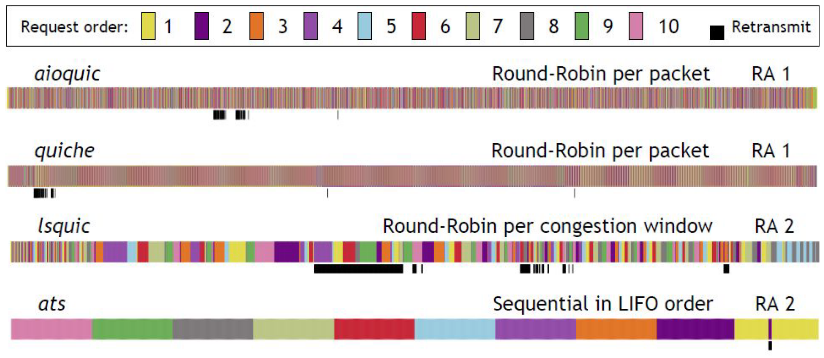
\includegraphics[width=0.5\textwidth]{images/Proto_differences_small.png}
%\caption{Comparison of QUIC connection request multiplexing for selected implementations, taken from \cite{marx2020same}.}
%\end{figure}
%
%
%\paragraph{7. Host level load}
%In a similar manner, other applications exhibiting significant computational load (CPU, memory, I/O) on the host machine can affect the processing speed of incoming and outgoing traffic, which can again alter IATs and the  overall duration of a connection. An example of this is visible in Fig. \ref{Fig:FTP_load}, where the host sends significantly less ack-packets when under heavy computational load. 
%%\textcolor{red}{Performed various experiments using \textit{stress} under sometimes enormous loads, the startup was a lot slower, but the traffic IATs etc did not change at all, but using Linux bridge and if going via loopback interface in the kernel stack}.
%
%\begin{figure}
%\centering
%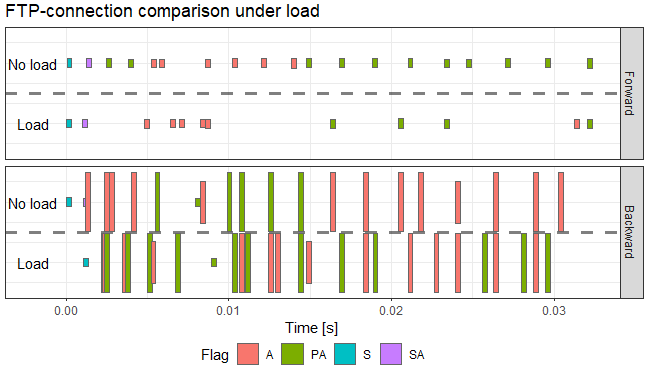
\includegraphics[width=0.5\textwidth]{images/FTP_load.png}
%\caption{Packet-sequence structure similarity comparison for FTP-activity under different load and otherwise constant settings. Colours indicate packet flags while the height of the packets indicates their size. Note that under load, the host sends significantly less packets.}\label{Fig:FTP_load}
%\end{figure}
%
%\paragraph{8. LAN and WAN congestion}
%Low available bandwith, long RTTs, or packet loss can have a significant effect on TCP congestion control mechanisms, which in turn influence frame-sizes, IATs, window sizes, and the overall temporal characteristic of the sequence. \textcolor{red}{do we need to verify this? Seems very clear}
%
%
%
%
%\vspace{0.3cm}
%We designed DetGen to control and monitor these factors in order to let researchers explore the impact of different aspects on their traffic models. We omitted some factors that can influence traffic structures, since these act either on a larger scale rather than micro-structures or correspond to \textcolor{red}{exotic} settings that are outside of our traffic generation scope. Among them are the following:
%
%
%
%
%\paragraph{1. User and scheduled activities}
%The choice and usage frequency of an application and task by a user governs the larger-scale temporal characteristic of a traffic capture. Since we are focusing on the traffic micro-structures here, we currently omit this impact factor from our analysis. 
%
%\paragraph{2. Networking stack load}
%TCP or IP queue filling of the kernel networking stack can increase packet waiting times and therefore IATs of the traffic trace, as shown by \cite{sequeira2013influence}. In practice, this effect seems to be constrained to large WAN-servers and routers, and we did not find any significant effect on the \textcolor{red}{described traffic similarity measures} for various amounts of load generated with iPerf for a regular UNIX host.
%
%
%%\paragraph{TCP congestion management implementation}
%%Different versions of the TCP congestion manager exist on Windows and Linux such as TCP Reno/Tahoe, which can have minor influence on the traffic, as shown by Grieco et al. \cite{grieco2004performance}. 
%%Existing implementations on a machine stay mostly constant, which is why we also omit this variable at the moment.
%% Implementations within a machine should stay constant.
%
%\paragraph{3. Network configurations}
%Network settings such as the MTU or the enabling of TCP Segment Reassembly Offloading have effects on the captured packet sizes, are standardised for most networks \textcolor{red}{where to find a proof for that?}.
%
%%but like TCP implementations stay mostly constant for a host.
%
%

%
%
%\section{Current data situation}
%
%Currently, intrusion detection researchers predominantly rely on public, synthetically generated datasets, on which NID systems are evaluated subsequently.
%\textit{Real-world datasets} such as LANL-15 \cite{kent-2015-cyberdata1} or UGR-16 \cite{macia2018ugr} provide the highest amount of traffic realism, but often lack detailed information such as packet captures due to privacy reasons, and give close to no information on the content of the provided data. 
%
%\textit{Synthetic datasets} such as the CICIDS-17 \cite{sharafaldin2018towards} or the UNSW-16  \cite{moustafa2015unsw} datasets are typically captured in virtual environments that simulate \textcolor{red}{commercial} networks with virtual machines. Traffic is generated from scripted activity, and attack data either injected or generated from carefully inserted vulnerabilities. The arranged settings normally lack the flexibility to generate customized data and by design only provide very limited attack diversity.
%%limited insights into the given traffic realism or 
%
%\textit{Attack traffic generators} typically aim at providing traces from a diverse set of attacks, and injecting them into existing traffic captures in various ways. Moirai \textcolor{red}{citation} for example calculates several quantitative characteristics to better embed the attack traffic.  However, most of the issues surrounding real-world traffic captures remain, and there is concern about the realism of injected attack traffic \textcolor{red}{citation}.
%
%Recently, some effort have been made to to generate completely artificial traffic data with \textit{generative adversarial networks} (GANs) trained on real-world traffic. While examples such as DoppelGANger or Ring et al. \textcolor{red}{citation} are successful at generating realistic large-scale network features such as activity levels or \textcolor{red}{connection graphs}, they are not aimed at intrusion detection and do not provide the necessary granularity to model connection- or packet-level features.
%
% \textit{Testbeds} such as Mininet offer tremendous \textcolor{red}{flexibility}, but are so far not targeted for intrusion detection and lack suitable small-scale traffic generation tools, labelling capabilities, or attack scenarios. 
%


%\section{Background and Motivation}
%
%%\subsection{Misuse and machine learning}
%
%
%%Network intrusion detection is the field of detecting intrusions in a network by analysing captured traffic traces exchanged between computers in the network. Most commonly used are misuse detection systems identify known signatures of bad behaviour in traffic such as malicious packet payloads or rule-based patterns concerning port usage and/or packet sequences. Although very efficient, these methods are reliant on precise details on known attacks in the form of signature databases. Significant efforts have been invested in developing machine-learning based methods that are trained on large amounts of traffic to develop a more generalisable distinction between benign and malicious behaviour to remove the need of attack signatures and enable the detection of zero-day attacks.
%
%
%%\subsection{Existing problems}
%
%Machine-learning based network intrusion detection has been subject to extensive criticism due to being unable to deliver sufficient detection rates at an acceptable false-positive rate in actual deployment. Two main causes for these failings have been identified particularly for network-based methods by Sommer and Paxson \cite{sommer2010outside} in 2010, which have been supported and partly extended by Harang \cite{harang2014bridging} in 2014 or by Liu et al. in 2019 \cite{liu2019machine}:
%
%
%\paragraph{Semantic gap between between results and their operational interpretation}
%
%Arguably the biggest concern expressed by Sommer and Paxson is that methods lack a deep semantic insight into a system's capabilities and limitations and are instead treated as black boxes. The authors here draw comparisons to other areas of machine learning such as character recognition where the precise understanding of the data structure and how existing systems process it have lead to breakthroughs such as the convolutional layers that process the data in a more adequate way. In network intrusion detection, different methods are thrown at existing data without thorough analysis where the system performs well and where it fails or breaks, and what the reasons for this are. The authors recommend to researchers to narrow the scope to more specific applications and closely examine what types of traffic trigger which responses by the system in order to develop a better understanding of where and how future systems can be designed to better suit this particular type of data and application. 
%
%
%%\begin{itemize}
%%%\item " To address them, we deem it crucial for any effective deployment to acquire deep, semanticinsightintoa system’s capabilities and limitations, rather than treatingthe system as a black box as unfortunately often seen."
%%
%%\item understanding the system’s semantic properties—the operationally relevantactivity that it can detect, as wellas theblind spotsevery system will necessarily have
%%
%%\item If we could give onlyonerecommendation on how toimprove the state of anomaly detection research, it would be:Understand what the system is doing
%%
%%\item an area whereinsightmatters much more than just numericalresults
%%
%%\item What can it detect, and why? What can itnot detect, and why not? How reliably does it operate?Where does it break?
%%
%%\end{itemize}
%
%
%\paragraph{Fundamental difficulties for conducting sound evaluation}
%
%The semantic gap stems in part from persistent difficulties for researchers to evaluate their system thoroughly and in a comparable and reproducible manner due to a lack of appropriate public datasets. Privacy and security concerns discourage network administrators to release rich and realistic datasets for the public,  leading to publicly available real-world datasets being the exception and missing informative features such as captured packets or consistent IP-addresses. This forces researchers to generate synthetic datasets using small virtual networks, and restricts the diversity and coverage of traffic researchers are able to examine.
%
%Furthermore, the labelling process is significantly more difficult in network intrusion detection than in other domains with easier interpretable data. Often, only traffic directly involved in an attack is labelled manually, with all other traffic receiving the same `Benign' label. This lack of informative labels impedes researchers abilities to analyse different types of traffic and thus understand the properties of their system.
%
%The lack of benchmark datasets often forces researchers to assemble their own data, which is mostly done in a non-reproducible way, leading to unverifiable detection rates and incomparable results.
%
%
%\vspace{0.2cm}
%Other problems identified by Sommer and Paxson include the diversity of network traffic, the high cost of errors, and lacking computational speed or detection systems.


\section{Conclusions}\label{Sec:Conclusion}

In this paper, demonstrated the impact of traffic generation with extensive micro-structure control as well as detailed corresponding documentation on researchers ability to evaluate and understand network intrusion detection models. We presented two use-cases in which we implemented and trained state-of-the art detection models before performing and detailed evaluation of their behaviour when encountering different traffic types. 

By using HTTP-traffic with congestion settings, we were quickly able to identify the inability of an LSTM-based classifier to handle traffic with significant retransmission rates, which enabled us to improve the model accordingly and increase detection performance by more than $2\%$. Similarly, the examination of projection consistency of a subspace-clustering method using traffic with artificially similar characteristics revealed an overly high sensitivity to flow interarrival times, while cluster-coherence could be increased significantly by identifying half-open connections that were dropped because of network failure as the source of overly dispersed traffic projections. 

These results should encourage researchers to perform more deep-going examinations of data-driven network intrusion detection models. It also shows that DetGen offers strong insights into traffic micro-structures and their effect on traffic models, and allows researchers to analyse the particular characteristics of events that lead to false-positives or model failure as well as their effect on model training.


%we proposed DetGen, a framework aimed at improving researchers understanding of traffic micro-structures and their respective effect on traffic models in order to close the \emph{semantic gap} described by Sommer and Paxson \cite{sommer2010outside}. DetGen allows reproducible traffic generation experiments that allow the control and monitoring different traffic shaping aspects while delivering data that is truthful to real-world structures. Our framework achieves this through containerised applications and corresponding process and traffic separation, meticulous attention to the corresponding generating activities and their facets, and the careful emulation and control of external effects. Currently, DetGen produces traffic for 29 different activities.

%We verified the improvements regarding reproducibility and traffic control of DetGen compared to traditional VM-setups in an experiment as well as the fidelity of the generated traffic to real-world characteristics in another experiment. Especially regarding the exclusion of background traffic and corresponding connection sequence structures, DetGen outperformed traditional setups significantly. In terms of traffic diversity, DetGen achieved significantly better results than current state-of-the-art NIDS-datasets.



%The major design advantages of this framework are the isolation of traffic scenarios into separate container arrangements, which allows the extension of new scenarios and detailed implementation of subscenarios as well as the capture of ground truth of the computational origins of individual traffic events. Furthermore, containerization enables the generation of traffic data at scale due to containers being light-weight and easily clonable.

%We verified the realism of the generated traffic and the corresponding ground truth information with two experiments, and demonstrated the usefulness of the framework in another experiment.
%Presently, our framework consists of 29 scenarios capable of producing benign and malicious network traffic. Several of these scenarios, such as the \emph{BitTorrent} or the \emph{Stepping-Stone} scenario, provide novel traffic data of protocols or behaviours that has not been widely available to researchers previously.


\subsection{Difficulties and limitations}

DetGen is building network traffic datasets from a small-scale level up by coalescing traffic from different fine-grained activities together. While this provides great insight into traffic micro-structures, our framework will not replicate realistic network-wide temporal structures, such as port usage distributions or long-term temporal activity. These quantities would have to be statistically estimated from other real-world traffic beforehand to allow our framework to emulate such behaviour reliably. Other datasets such as UGR-16 use this approach to fuse real-world and synthetic traffic and are currently better suited to build models of large-scale traffic structures.

Furthermore, while controlling traffic shaping factors artificially helps at identifying the limits and weak points of a model, it can exaggerate some characteristics in unrealistic ways and thus both affect the training phase of a model as well as tilt the actual detection performance of a model in either direction. Additionally, the artificial randomisation of traffic shaping factors can currently not generate the traffic diversity encountered in real-life traffic and thus only aid at exploring model limits extensively. The lack of realistic traffic heterogeneity however is at the moment significantly more pronounced in commonly used network intrusion datasets such as the CICIDS-17 dataset, where the vast majority of successful FTP-transfers consist of a client downloading a single text file that contains the Wikipedia page for ‘Encryption’ \textcolor{red}{insert DetGen citation}.

%We paid meticulous attention to enable control over as many traffic impact factors as possible. However, DetGen is currently only offering insufficient control over underlying application-layer implementations such as TLS 1.3 vs 1.2. In theory, it should be unproblematic to provide containers with different implementations for each scenario to provide this control. However we faced difficulties to compile containers in a suitable manner and are currently investigating, how to improve DetGen on this shortcoming.

%Working with Docker containers can sometimes complicate the implementation of individual scenarios compared to working with VMs. Although several applications are officially maintained Docker containers that are free from major errors, many do not. For instance, in the \textit{BitTorrent} scenario, most common command line tools, such as \texttt{mktorrent}, \texttt{ctorrent} and \texttt{buildtorrent}, failed to actually produce functioning torrent files from within a container due to Docker's union filesystem. Furthermore, due to the unique way in which we are using these software packages, unusual configuration settings are sometimes needed. %As such, many 

%Lastly, capturing \texttt{.pcap}-files from each container can quickly exceed available disc space when generating traffic at scale. Depending on specific research requirements, it is advizable to add filtering or feature extraction commands to the scenario execution scripts to enable traffic preprocessing in real-time.


\subsection{Future work}

Our traffic generation framework is designed to be expandable and there are many avenues for future work. The continual development of scenarios and subscenarios would improve the potential realism of datasets generated using the framework. The addition of more malicious scenarios would enable a more detailed model evaluation and improve detection rate estimation. 
Another future improvement for framework is to add scripts that emulate the usage activity of individual scenarios by a user or a network. 


%Although ground truth for particular traffic traces is provided by capturing \texttt{.pcap}-files for each container individually, we have not implemented a labelling mechanism yet for the dataset coalescence process. Though not technically difficult, some thought will have to be put how such labels would look like to satisfy different research demands.
Furthermore, the Docker platform provides the functionality to collect system logs via the \texttt{syslog logging driver}. We plan on implementing their collection in the future, where they could act either as traffic labels providing more ground truth details, or act as a separate data source that complements the collected traffic.

We wish to publish this framework to a wider audience, allowing for further modification. This will be done using a GitHub repository, which contains both the implemented capture scenarios as well as the corresponding container images.



%We are grateful for our ongoing collaboration with our industry partners  on this topic area, who provided both ongoing support and guidance to this work. Discussions with them have helped reinforce the need for a better evaluation and understanding of the possibilities that new intelligent tools can provide.

%Full funding sources after currently blinded.

\bibliographystyle{abbrv}
 
\bibliography{../DetGen_ext}

%\appendix


\end{document}
